%! TEX root = ./Equipo 1 - cuarto corte.tex
\documentclass[lettersize,journal]{IEEEtran}

\usepackage{amsmath,amsfonts}
\usepackage{array}
\usepackage[caption=false,font=footnotesize]{subfig}
\usepackage{textcomp}
%\usepackage{stfloats}
\usepackage{url}
\usepackage{graphicx}
\usepackage{cite}
\usepackage{xcolor}
\usepackage{algorithm}
\usepackage{algpseudocode}
\usepackage{booktabs}
\usepackage{tikz}
\usetikzlibrary{shapes.geometric,arrows.meta,positioning,fit,backgrounds}
%\usepackage{enumitem}
\usepackage{placeins}
\graphicspath{{figures/}}
\usepackage{balance}
\renewcommand{\ttdefault}{cmtt}
\begin{document}
	
	%=================================================================
	\title{SOFIA: Modular Robotic Kinetic Surface for Human-Robot Interaction and Thermal-Constrained Actuator Characterization}
	
	\author{Paola M. Covarrubias-Viveros, Lizeth A. M{\'e}ndez-Ortiz, Juan Bernardo Orozco-Quirarte, Karen I. S{\'a}nchez-Garc{\'\i}a, Alan E. Fuentes-Guti{\'e}rrez, Jorge A. Lizarraga, Graciela Baca, Luis Enrique Gonz{\'a}lez-Jim{\'e}nez and Luis F. Luque-Vega
		\thanks{The authors are with the Department of Electronics, Systems and
			Informatics (DESI), ITESO, Tlaquepaque 45604, Jalisco, Mexico.}}
	
	\markboth{LabDST SOFIA, ITESO, Fall 2026}%
	{Covarrubias-Viveros \MakeLowercase{\textit{et al.}}: SOFIA: Modular Robotic Kinetic Surface}
	
	\maketitle
	
	%=================================================================
	\begin{abstract}
		Modular robotic systems leverage repeatable electromechanical units to enable flexible, scalable, and reconfigurable architectures. In interactive human-robot installations, spatial tracking of human body posture and gestures provides intuitive stimulus-response dynamics. \linelabel{ln:abs}This paper presents the modular design, end-to-end physical integration, and experimental validation of SOFIA, an interactive kinetic surface comprising sixteen electromechanical units, each providing two rotational degrees of freedom actuated by commercial MG90S servomotors. While commercial servomotors encapsulate internal closed-loop position control via pulse-width modulation (PWM), persistent angular errors caused by mechanical stalls, external disturbances, or fabrication tolerances induce thermal degradation and excessive power consumption. \linelabel{ln:abs-inv}To investigate actuator reliability under persistent position error conditions, this work formulates an experimental characterization protocol assessing the electrothermal response of an MG90S under mechanical stall. Using an LM35 precision temperature sensor and an INA219 current monitor, actuator heating is characterized during continuous stall ($\bar{I}_{\text{stall}} = 861.8 \pm 181.4\text{ mA}$, $\bar{P} = 4.07\text{ W}$), \linelabel{ln:abs-tau}revealing a mean heating rate of $\bar{\beta}_1 = 0.214\,^\circ\text{C/s}$ ($R^2 = 0.993$; initial $60\text{ s}$ slope $0.111\,^\circ\text{C/s}$) in Trial~1 and a peak temperature at stall release of $70.21^\circ\text{C}$ in extended testing (Trial~2) prior to thermal equilibrium. \linelabel{ln:abs-claim}Furthermore, a real-time 30~FPS MediaPipe 3D gesture recognition pipeline is integrated with the physical ESP32-C3 prototype via a fault-tolerant bidirectional BLE protocol (\texttt{\$SEQ,CMD\#}) supporting seven interactive postures, automatic hardware reconnection, and stress-tested immunity against rapid transition chattering, multi-user spatial conflict, and variable illumination.
	\end{abstract}
	
	\begin{IEEEkeywords}
		Modular robotics, human-robot interaction (HRI), servomotor thermal characterization, actuator saturation, computer vision, inverse kinematics.
	\end{IEEEkeywords}
	
	%=================================================================
	\section{Introduction}
	\label{sec:introduction}
	
	\IEEEPARstart{M}{odular} \linelabel{ln:intro1}robotics enables constructing complex spatial mechanisms from repeatable functional units integrating mechanical, electronic, and control capabilities, offering superior reconfigurability and maintainability over monolithic robotic architectures~\cite{seo2019modular}.
	
	\linelabel{ln:intro-hri}In parallel, socially interactive and human-robot interaction (HRI) systems incorporate perception and actuation mechanisms to establish continuous, non-verbal dialogue with human participants. Within this domain, posture, gestures, and body kinematics constitute vital communication channels for interpreting user intent and synthesizing reactive robotic behavior~\cite{fong2003social}. Consequently, modern kinetic robotic installations operate not merely as automated spatial mechanisms, but as interactive expressive surfaces capable of responding synchronously to multimodal human stimuli.
	
	\linelabel{ln:intro-sofia}Within this framework, this paper introduces SOFIA, a modular robotic installation comprising sixteen electromechanical units arranged in a kinetic honeycomb array. Each module provides two rotational degrees of freedom (2-DOF) driven by dual metal-gear MG90S servomotors (32 actuators total). \linelabel{ln:intro-onboard}Actuator control and signal distribution are organized through a centralized electronic architecture, wherein a master ESP32-C3 processing node manages trajectory interpolation and commands dual 16-channel PCA9685 PWM drivers over an I$^2$C bus to synchronously synthesize the 32 servo control pulses. Supervisory communication is established via Bluetooth Low Energy (BLE) and Wi-Fi, with hardware provision for inter-module expansion over an industrial RS-485 / Modbus bus.
	
	\linelabel{ln:intro-hw}The system relies on the ESP32-C3 microcontroller as the core processing and telemetry engine~\cite{espressif2024esp32c3}, coupled with PCA9685 16-channel 12-bit I$^2$C PWM controllers~\cite{nxp2015pca9685} to synthesize precise 50~Hz control pulses for the servomotors. Although commercial off-the-shelf (COTS) servomotors simplify spatial positioning, their internal closed-loop controllers remain completely encapsulated within the actuator housing. Consequently, while the supervisory system commands an angular setpoint via external 50~Hz PWM duty cycles, the internal drive strategy utilized to eliminate error between reference and actual shaft position is inaccessible to the designer.
	
	\linelabel{ln:intro-stall}This characteristic becomes critical when a servomotor experiences operational constraints where it cannot reach the commanded angular setpoint. In large-scale kinetic arrays composed of numerous densely packed modules, mechanical interference, fabrication tolerances, structural interference, or physical obstacles produce persistent, non-zero position errors. Under such conditions, internal driver behavior governs current draw, internal thermal dissipation, and long-term hardware reliability.
	
	\linelabel{ln:intro-bb}When a bounded-input actuator experiences persistent saturation~\cite{kirk2004optimal}, \linelabel{ln:intro-boyd}analyzing its response across distinct motion and mechanical load regimes requires joint electrical current and surface temperature telemetry.
	
	\linelabel{ln:intro-obj}To address this challenge, this paper experimentally characterizes the electromechanical and thermal behavior of the MG90S servomotor under persistent position error. By imposing a mechanical constraint on the output shaft and monitoring surface temperature with a precision LM35 sensor, this study extracts empirical first-order thermal models via linear regression. \linelabel{ln:hyp}The primary working hypothesis posits that persistent angular error induces an observable thermal signature that quantitatively reflects actuator operational constraints. \linelabel{ln:rq}Accordingly, the central research question guiding this work is: \textit{Does persistent position error in an MG90S servomotor produce an identifiable thermal signature that bounds the safe holding time of a SOFIA kinetic module?} To answer this question, four specific, measurable technical objectives are addressed:
	\begin{enumerate}
		\setlength{\itemsep}{0pt}
		\setlength{\parskip}{0pt}
		\setlength{\parsep}{0pt}
		\item \linelabel{ln:obj-act}\textbf{Actuator Evaluation:} Quantify raw mechanical travel ($\Delta q_{\max} \ge 50^\circ$, bounded in operation to $q_j^{\text{servo}} \in [60^\circ, 120^\circ]$), quiescent dead-band current ($I_{\text{quiesc}} \le 5\text{ mA}$), and active $60^\circ$ transit pulse duration ($\le 100\text{ ms}$) under $50\text{ Hz}$ PWM drive.
		\item \linelabel{ln:obj-therm}\textbf{Thermal Modeling:} Characterize locked-rotor stall heating to identify the empirical heating rate ($R^2 \ge 0.95$) and derive a safety dwell timeout maintaining casing temperature $T_s \le T_{\text{safe}} = 60^\circ\text{C}$.
		\item \linelabel{ln:obj-vis}\textbf{Perception and Telemetry Validation:} Extract 3D pose and 21-point hand landmarks via MediaPipe at $\le 33\text{ ms}$ frame budget ($30\text{ FPS}$), verify end-to-end 7-posture triggering and fault-rejection in the framed BLE protocol (\texttt{\$SEQ,CMD\#}), and bound nominal actuation response $\le 250\text{ ms}$.
		\item \linelabel{ln:obj-kin}\textbf{Kinematic Simulation:} Formulate closed-form 2-DOF analytical kinematics and verify 16-module inverse-kinematics consistency ($\varepsilon_\psi \le 0.5^\circ$ in-cone) and wide-sweep clamped error $\text{MAE} \le 3.5^\circ$ (below a $5^\circ$ visual misalignment threshold at $1\text{ m}$).
	\end{enumerate}
	\linelabel{ln:contrib}Unlike robotic interaction systems that rely on bounding-box object detection and discrete actuator control, SOFIA integrates 3D geometric hand estimation via MediaPipe Hand Landmarker with the control of 2-DOF robotic modules driven by MG90S servomotors. Furthermore, it incorporates an experimental characterization of the servomotors across distinct operating conditions, evaluating their electrical and thermal behavior from current and temperature measurements to analyze their response under varying motion and mechanical load conditions and identify operational limitations \linelabel{ln:contrib-claim}intended to support reliable kinetic surfaces.
	
	\subsection{Related Work}
	\label{sec:related_work}
	
	\linelabel{ln:rw1}Recent advances in interactive surfaces and vision-driven robotics have accelerated with lightweight machine learning inference frameworks. Qui{\~n}onez \textit{et al.}~\cite{quinonez2022mediapipe} and Lugaresi \textit{et al.}~\cite{lugaresi2019mediapipe} demonstrated the efficacy of MediaPipe perception graphs for real-time 3D landmark estimation, which, combined with optimized computer vision pipelines via OpenCV~\cite{bradski2000opencv}, enable 21-point hand skeleton topologies to be extracted with minimal computational latency.
	
	\linelabel{ln:rw2}In the domain of dynamic physical interfaces and shape displays, Follmer \textit{et al.}~\cite{follmer2013inform} introduced inFORM, a 2.5D shape display comprising 900 motorized linear pins operating at high update rates for dynamic tangible interaction. Expanding toward interactive kinetic architectural furniture, Nakagaki \textit{et al.}~\cite{nakagaki2016transform} developed Transform, incorporating over 1,000 independent motorized linkages. In modular and reconfigurable robotics, Seo \textit{et al.}~\cite{seo2019modular} formalized scalability criteria, distributed communication, and power distribution across repeatable electromechanical units, while Fong \textit{et al.}~\cite{fong2003social} surveyed social robotics, demonstrating that physical motion, non-verbal mirroring, and gestural responsiveness enhance user engagement.
	
	\begin{table}[!t]
		\centering
		\caption{Benchmarking Comparison of Interactive Kinetic Surfaces and Shape Displays}
		\label{tab:benchmarking}
		\scriptsize
		\setlength{\tabcolsep}{2pt}
		\renewcommand{\arraystretch}{0.92}
		\begin{tabular}{@{}p{1.35cm} p{1.05cm} p{1.15cm} p{1.45cm} p{2.45cm}@{}}
			\toprule
			\textbf{Platform} & \textbf{Units (DOF)} & \textbf{Range / DOF} & \textbf{Actuator Type} & \textbf{Latency / Update Rate} \\
			\midrule
			inFORM~\cite{follmer2013inform} & 900 (1-DOF) & $100\text{ mm}$ (linear) & DC motorized pin & $\approx 16.7\text{ ms}$ ($60\text{ Hz}$); optical $\approx 70\text{ ms}$ \\
			Transform~\cite{nakagaki2016transform} & 1,152 (1-DOF) & $100\text{ mm}$ (linear) & DC gearmotor & $\approx 33.3\text{ ms}$ ($30\text{ Hz}$) \\
			\textbf{SOFIA (Ours)} & \textbf{16 (2-DOF)} & $\mathbf{\pm 30^\circ}$ ($\mathbf{60^\circ\text{--}120^\circ}$) & \textbf{Metal MG90S} & \textbf{5~Hz BLE stream;}\newline\textbf{100--180~ms slew}$^{\mathrm{a}}$ \\
			\bottomrule
			\multicolumn{5}{@{}p{7.6cm}@{}}{\vspace{2pt}\footnotesize $^{\mathrm{a}}$Nominal $60^\circ$ servo slewing ($100\text{--}180\text{ ms}$ datasheet) with $\le 0.12\text{ ms}$ PC logic latency; statistical BLE RTT and optical test pending.}
		\end{tabular}
	\end{table}
	
	\linelabel{ln:rw-gap}Despite these advances, existing kinetic installations and shape displays~\cite{follmer2013inform,nakagaki2016transform,seo2019modular} predominantly assume ideal actuator trajectory completion, frequently overlooking actuator stall dynamics, current surges, and internal thermal accumulation occurring across densely populated arrays. While classical optimal control formulations~\cite{kirk2004optimal} establish theoretical boundaries for bounded controller actions, physical implementations require empirical thermal validation; building upon these foundations, this research bridges the gap between high-level visual tracking and low-level physical actuator reliability.
	
	\subsection{Demonstrator Analysis}
	\label{sec:demonstrator_analysis}
	
	\begin{table}[!t]
		\centering
		\caption{Functional Decomposition Matrix of the SOFIA Demonstrator Module}
		\label{tab:functional_matrix}
		\scriptsize
		\setlength{\tabcolsep}{2pt}
		\renewcommand{\arraystretch}{0.92}
		\begin{tabular}{@{}p{1.2cm} p{1.8cm} p{1.35cm} p{1.45cm} p{1.85cm}@{}}
			\toprule
			\textbf{Subsystem} & \textbf{Function} & \textbf{Input} & \textbf{Output} & \textbf{Limitation} \\
			\midrule
			Perception & Hand landmark tracking & RGB video stream & 3D normalized coordinates & Occlusion, ambient lighting \\
			Control / Telemetry & Trajectory interpolation & BLE / Modbus packets & Target angle $\theta_d(t)$ & Bus contention, latency \\
			Actuation & 2-DOF angular orientation & 50~Hz PWM duty cycle & Shaft angle $\theta(t)$, torque & Stall heating, unobservable $e(t)$ \\
			Kinematic Core & Planar honeycomb articulation & Dual servo shaft torque & Spatial facet tilt & Angular range limits ($19.3^\circ$--$70.2^\circ$) \\
			Power / Thermal & Regulated current delivery & 5.0~V DC bus & Electrical power & Joule dissipation, no active cooling \\
			\bottomrule
		\end{tabular}
	\end{table}
	
	\begin{table*}[!t]
		\centering
		\caption{Bill of Materials Summary for the SOFIA 16-Module Robotic Surface}
		\label{tab:bom_sofia}
		\scriptsize
		\renewcommand{\arraystretch}{0.86}
		\begin{tabular}{p{3.2cm} c c p{5.0cm} p{2.8cm} p{2.5cm}}
			\toprule
			\textbf{Component} & \textbf{Unit} & \textbf{Sys.} & \textbf{Technical Description} & \textbf{Manufacturer} & \textbf{Location} \\
			\midrule
			MG90S Servomotor & 2 & 32 & Metal-gear micro servo, 1.8--2.2~kgf$\cdot$cm, 50~Hz PWM & TowerPro & Shenzhen, China \\
			Module Enclosure & 1 & 16 & 3D-printed PLA honeycomb casing (SOFIA003) & In-house (LabDST) & Tlaquepaque, MX \\
			M3 Fasteners & 4 & 64 & Stainless steel socket cap screw, M3 $\times$ 10~mm & Generic & Tlaquepaque, MX \\
			PCA9685 Driver & -- & 2 & 16-ch 12-bit I$^2$C PWM driver breakout (32 ch total) & UNIT Electronics & Mexico City, MX \\
			ESP32-C3 MCU & -- & 1 & 32-bit RISC-V Super Mini, Wi-Fi / BLE 5.0 & Espressif & Shanghai, China \\
			RS-485 Transceiver & -- & 2 & MAX485 / SP3485 differential bus transceiver & Maxim / Generic & San Jose, USA \\
			JST-VH Connectors & 2 & 32 & 2-pin 3.96~mm high-current servo supply connector & J.S.T. Mfg. Co. & Tokyo, Japan \\
			Power Supply (PSU) & -- & 1 & Regulated 5.0~V / 20~A (100~W, LRS-100-5) & Mean Well & New Taipei, TW \\
			Decoupling Caps & 1 & 16 & Low-ESR electrolytic, $2200\,\mu\text{F}$, 16~V per branch & Nichicon / Generic & Kyoto, Japan \\
			Prototyping PCB & -- & 1 & Power distribution and signal routing carrier & In-house / Generic & Tlaquepaque, MX \\
			Wiring Harness & 2 & 32 & 14~AWG trunk ($1.5\text{ m}$ RT) + 22~AWG leads ($0.70\text{ m}$ RT) & Generic & Tlaquepaque, MX \\
			INA219 Sensor & -- & 2 & I$^2$C bidirectional current/power monitor ($10\text{ m}\Omega$) & TI / UNIT & Mexico City, MX \\
			LM35 Sensor & 1 & 1 & Analog temperature sensor ($10\text{ mV}/^\circ\text{C}$), test bench & TI / UNIT & Mexico City, MX \\
			\bottomrule
		\end{tabular}
	\end{table*}
	
	\linelabel{ln:demo-intro}During the initial \textit{Discover} stage of the D-Lab methodology, guided physical observation of the SOFIA proof-of-concept module identified critical operational failure modes emerging from dense actuator packaging. The modular kinetic cell decomposes into five core functional subsystems, summarized in the functional decomposition matrix (Table~\ref{tab:functional_matrix}).
	
	\linelabel{ln:demo-obs}Guided laboratory observations revealed that during spatial multi-facet alignment, adjacent 3D-printed petals occasionally encounter mechanical interference due to fabrication tolerances ($\pm 0.4\text{ mm}$) and rapid user gesture transients. Consequently, actuators become physically constrained before achieving commanded setpoints. 
	
	To structure\linelabel{ln:demo-tree} this vulnerability, Fig.~\ref{fig:problem_tree} synthesizes the D-Lab problem tree linking the three underlying root causes (unmonitored shaft position, continuous H-bridge saturation under error, and enclosed modular housings) to the core focal problem—persistent angular tracking error $e(t) = \theta_d(t) - \theta_{\text{stall}} \neq 0$—and its direct system-level effects. These findings motivated the experimental thermal characterization and bounded control strategies developed in this work.
	
	\begin{figure}[!t]
		\centering
		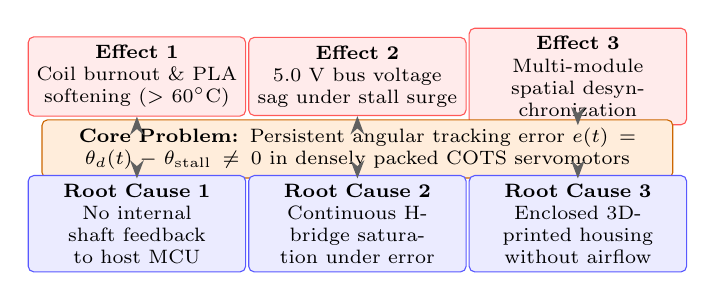
\begin{tikzpicture}[
			>=Stealth,
			box/.style={draw, rectangle, rounded corners=2pt, align=center, font=\scriptsize, inner sep=3pt},
			eff/.style={box, fill=red!8, draw=red!65, text width=2.55cm, minimum height=0.72cm},
			core/.style={box, fill=orange!14, draw=orange!80!black, text width=7.8cm, minimum height=0.65cm},
			root/.style={box, fill=blue!8, draw=blue!65, text width=2.55cm, minimum height=0.78cm},
			arr/.style={->, thick, gray!75!black}
			]
			% Direct Effects (Top)
			\node[eff] (e1) at (-2.8, 0.92) {\textbf{Effect 1}\\Coil burnout \& PLA softening ($>60^\circ\text{C}$)};
			\node[eff] (e2) at (0, 0.92) {\textbf{Effect 2}\\5.0~V bus voltage sag under stall surge};
			\node[eff] (e3) at (2.8, 0.92) {\textbf{Effect 3}\\Multi-module spatial desynchronization};
			
			% Core Problem (Center)
			\node[core] (core) at (0, 0) {\textbf{Core Problem:} Persistent angular tracking error $e(t) = \theta_d(t) - \theta_{\text{stall}} \neq 0$ in densely packed COTS servomotors};
			
			% Root Causes (Bottom)
			\node[root] (r1) at (-2.8, -0.95) {\textbf{Root Cause 1}\\No internal shaft feedback to host MCU};
			\node[root] (r2) at (0, -0.95) {\textbf{Root Cause 2}\\Continuous H-bridge saturation under error};
			\node[root] (r3) at (2.8, -0.95) {\textbf{Root Cause 3}\\Enclosed 3D-printed housing without airflow};
			
			\draw[arr] (r1.north) -- (core.south -| r1.north);
			\draw[arr] (r2.north) -- (core.south);
			\draw[arr] (r3.north) -- (core.south -| r3.north);
			\draw[arr] (core.north -| e1.south) -- (e1.south);
			\draw[arr] (core.north) -- (e2.south);
			\draw[arr] (core.north -| e3.south) -- (e3.south);
		\end{tikzpicture}
		\caption{Problem tree analysis synthesized during the D-Lab Discover stage, mapping root causes to persistent position error and system-level effects.}
		\label{fig:problem_tree}
	\end{figure}
	
	\subsection{Formal Problem Formulation}
	\label{sec:problem_formulation}
	
	\linelabel{ln:pf}The SOFIA system requires coordinated spatial orientation of 32 independent servomotors across 16 electromechanical modules. Each actuator receives an angular reference setpoint $\theta_d(t)$ and is commanded to achieve the target physical orientation $\theta(t)$.
	
	\linelabel{ln:pf-e}The angular position error $e(t)$ for any given actuator is formally defined as:
	\begin{equation}
		e(t) = \theta_d(t) - \theta(t),
		\label{eq:position_error}
	\end{equation}
	where $\theta_d(t) \in [\theta_{\min}, \theta_{\max}]$ corresponds to the desired (commanded) angular position, and $\theta(t)$ denotes the instantaneous actual angular position of the output shaft. In the single-axis experimental characterization, the scalar variable $\theta(t) \equiv q_j(t)$ ($j \in \{1, 2\}$) denotes the coordinate of the servomotor under test, corresponding identically to either joint axis of the 2-DOF kinetic module.
	
	\linelabel{ln:pf-ts}Under ideal, unconstrained operation, the internal feedback loop drives $e(t) \to 0$ within a settling time $t_s \in [75, 180]\text{ ms}$. However, when an external mechanical constraint prevents the actuator from reaching $\theta_d(t)$ such that $\theta(t) = \theta_{\text{stall}} \neq \theta_d(t)$, the error persists indefinitely:
	\begin{equation}
		e(t) = \theta_d(t) - \theta_{\text{stall}} = \Delta\theta_0 \neq 0, \quad \forall t \ge t_0.
		\label{eq:persistent_error}
	\end{equation}
	
	When $e(t)$ \linelabel{ln:pf-hbridge}persists, the internal H-bridge driver continuously supplies high current to the DC coreless motor in an attempt to minimize the tracking discrepancy. This condition causes significant Joule heating ($P_{\text{loss}} = I^2 R$) within the motor armature and driver silicon, inducing rapid thermal accumulation. Modeling this thermal profile and its associated time constant provides the quantitative foundation for actuator risk mitigation in the SOFIA array.
	
	%=================================================================
	\section{Materials and Methods}
	\label{sec:methods}
	
	\linelabel{ln:r3-7-req}To establish traceable verification criteria across the electromechanical, electronic, and software tiers, Table~\ref{tab:system_requirements} defines the six core system requirement categories (\texttt{REQ-PWR}, \texttt{REQ-MEC}, \texttt{REQ-CTL}, \texttt{REQ-COM}, \texttt{REQ-SAF}, and \texttt{REQ-ENV}) along with their quantitative acceptance thresholds. Table~\ref{tab:bom_sofia} \linelabel{ln:bom}summarizes the bill of materials for the SOFIA 16-module system, including each component's technical description, manufacturer, and country of origin. Furthermore, \linelabel{ln:r1-1-cite}Table~\ref{tab:compliance} evaluates the critical parameters of each key component against the requirements defined in Table~\ref{tab:system_requirements}, distinguishing verified compliance (\textit{Compliant}) from array-level items under assembly (\textit{Pending}).
	
	\begin{table}[!t]
		\centering
		\caption{SOFIA System Requirements and Quantitative Acceptance Criteria}
		\label{tab:system_requirements}
		\scriptsize
		\setlength{\tabcolsep}{3pt}
		\renewcommand{\arraystretch}{0.88}
		\begin{tabular}{@{}l p{2.3cm} p{4.6cm}@{}}
			\toprule
			\textbf{Req. ID} & \textbf{Category} & \textbf{Measurable Acceptance Criterion} \\
			\midrule
			\texttt{REQ-PWR} & Power Distribution & Regulated $5.0\text{ V}$ servo rail ($V_{\text{rail}} \ge 4.75\text{ V}$, $\Delta V \le 0.25\text{ V}$) and $3.3\text{ V}$ logic rail ($\ge 0.5\text{ A}$) with common ground. \\
			\texttt{REQ-MEC} & Mechanical / Torque & Actuator stall torque $\ge 3\times$ static facet load ($\tau_{\text{req}} \approx 0.45\text{ kgf}\cdot\text{cm}$ for $m_f = 28\text{ g}$, $r_{\text{cg}} = 1.5\text{ cm}$); collision-free travel $q_j^{\text{servo}} \in [60^\circ, 120^\circ]$. \\
			\texttt{REQ-CTL} & Motion Control & $50\text{ Hz}$ PWM resolution $\le 0.1^\circ$; $60^\circ$ slewing time $\le 180\text{ ms}$; dead-band $\le 5\,\mu\text{s}$. \\
			\texttt{REQ-COM} & Telemetry / Bus & Bidirectional BLE link ($\text{RTT} \le 50\text{ ms}$, $200\text{ ms}$ timeout, auto-reconnect) and Fast-mode I$^2$C ($400\text{ kHz}$). \\
			\texttt{REQ-SAF} & Thermal Safety & Casing temperature $T_s \le T_{\text{safe}} = 60^\circ\text{C}$ (below $65^\circ\text{C}$ PLA/retainer softening) via $\Delta t \le 15\text{ s}$ command timeout. \\
			\texttt{REQ-ENV} & Environmental & Component operating temperature range spanning $0^\circ\text{C}$ to $+70^\circ\text{C}$ inside enclosed PLA modules. \\
			\bottomrule
		\end{tabular}
	\end{table}
	
	\begin{table*}[!t]
		\centering
		\caption{Component Technical Specifications and System Requirements Compliance Assessment}
		\label{tab:compliance}
		\scriptsize
		\renewcommand{\arraystretch}{0.86}
		\begin{tabular}{p{1.7cm} p{2.3cm} p{2.9cm} p{3.4cm} c c p{3.1cm}}
			\toprule
			\textbf{Component} & \textbf{Parameter} & \textbf{Nominal / Measured Value} & \textbf{System Justification (Requirement)} & \textbf{Evid.} & \textbf{Status} & \textbf{Verification Source} \\
			\midrule
			\multicolumn{7}{l}{\textbf{ESP32-C3 Master Microcontroller (Espressif Systems)}} \\
			ESP32-C3 & Supply Voltage & 3.0--3.6~V (3.3~V typical) & \texttt{REQ-PWR}: Regulated logic rail operation & Datasheet & Compliant & Datasheet v2.4, Sec. 5.2 \\
			ESP32-C3 & Supply Current & 0.5~A minimum rating & \texttt{REQ-PWR}: Core and radio headroom & Datasheet & Compliant & Datasheet v2.4, Sec. 5.2 \\
			ESP32-C3 & Wi-Fi / BLE Peak & 276--335~mA peak & \texttt{REQ-COM}: RF burst capacity & Datasheet & Compliant & Datasheet v2.4, Sec. 5.6.1 \\
			ESP32-C3 & Logic VIH / VIL & $\ge 0.75\text{VDD}$ / $\le 0.25\text{VDD}$ & \texttt{REQ-CTL}: $3.3\text{ V}$ I$^2$C noise margins & Datasheet & Compliant & Datasheet v2.4, Sec. 5.4 \\
			ESP32-C3 & Boot Strapping & GPIO2, GPIO8, GPIO9 & \texttt{REQ-CTL}: Deterministic flash boot & Datasheet & Compliant & Datasheet v2.4, Sec. 3.1 \\
			ESP32-C3 & Wireless Link & 2.4~GHz Wi-Fi / BLE 5.0 & \texttt{REQ-COM}: Framed GATT link ($200\text{ ms}$ timeout) & Measured & Compliant & \texttt{registro\_pruebas\_ciclo.csv} \\
			ESP32-C3 & Operating Temp. & $-40^\circ\text{C}$ to $+85^\circ\text{C}$ (FN4) & \texttt{REQ-ENV}: Enclosed PLA module & Datasheet & Compliant & Datasheet v2.4, Sec. 1.2 \\
			\midrule
			\multicolumn{7}{l}{\textbf{MG90S Metal-Gear Micro Servomotor (TowerPro)}} \\
			MG90S & Supply Voltage & 4.8--6.0~V DC & \texttt{REQ-PWR}: Regulated 5.0~V rail & Datasheet & Compliant & Datasheet, TowerPro, p. 2 \\
			MG90S & Stall Torque & 1.8~kgf$\cdot$cm (4.8~V), 2.2 (6.0~V) & \texttt{REQ-MEC}: $>4\times$ dynamic load ($0.45\text{ kgf}\cdot\text{cm}$) & Datasheet & Compliant & Datasheet, p. 1 \& CAD calc \\
			MG90S & Operating Speed & 0.10~s$/60^\circ$ (4.8~V), 0.08 (6.0~V) & \texttt{REQ-CTL}: Nominal $60^\circ$ slew $\le 100\text{ ms}$ & Datasheet & Compliant & Datasheet, TowerPro, p. 1 \\
			MG90S & Control Signal & 50~Hz PWM, 1.0--2.0~ms & \texttt{REQ-CTL}: PCA9685 compatibility & Datasheet & Compliant & Datasheet, TowerPro, p. 2 \\
			MG90S & Dead Band & $5\,\mu\text{s}$ ($I_{\text{quiesc}} = 3.12\text{ mA}$) & \texttt{REQ-CTL}: Quiescent hold & Meas.+DS & Compliant & \texttt{datos\_5grados.csv} \\
			MG90S & Evaluated Angle & Raw $[19.3^\circ, 70.2^\circ]$; cmd $[60^\circ, 120^\circ]$ & \texttt{REQ-MEC}: $\pm 30^\circ$ travel around $90^\circ$ & Measured & Compliant & \texttt{servo\_characterization.xlsx} \\
			MG90S & Transient Pulse & $\le 100\text{ ms}$ (1--2 samples at $20\text{ Hz}$) & \texttt{REQ-CTL}: $60\text{ FPS}$ optical test & Pending & Pending & \texttt{datos\_901.csv}; optical pending \\
			MG90S & Stall Current & $861.8 \pm 181.4\text{ mA}$ ($39\text{--}311\text{ s}$) & \texttt{REQ-PWR}: PSU sizing ($20\text{ A}$) & Measured & Compliant & \texttt{datos\_CHIDOS\_DE\_FORZADO.csv} \\
			MG90S & Thermal Limit & Safe limit $T_{\text{safe}} \le 60^\circ\text{C}$ & \texttt{REQ-SAF}: Dwell timeout ($\Delta t \le 15\text{ s}$) & Pending & Pending & Firmware dwell; thermal cut-off pending \\
			MG90S & Packaging / Mass & 22.5 $\times$ 12 $\times$ 35.5~mm, 13.4~g & \texttt{REQ-MEC}: Fit in 2-DOF gimbal & Datasheet & Compliant & Datasheet, TowerPro, p. 1 \\
			\midrule
			\multicolumn{7}{l}{\textbf{PCA9685 16-Channel 12-Bit PWM Controller (NXP Semiconductors / UNIT Electronics)}} \\
			PCA9685 & Supply Voltage & 2.3--5.5~V DC ($3.3\text{ V }\text{V}_{\text{CC}}$) & \texttt{REQ-PWR}: Logic compatibility & Datasheet & Compliant & Datasheet Rev. 4, Table 14 \\
			PCA9685 & PWM Resolution & 12-bit (4096 steps, $\approx 0.04^\circ$) & \texttt{REQ-CTL}: Fine angular step & Datasheet & Compliant & Datasheet Rev. 4, Sec. 1 \\
			PCA9685 & Channel Cap. & 16 independent PWM outputs & \texttt{REQ-CTL}: 1 module tested; 32-ch PCB & Pending & Pending & 2-ch verified; 32-ch PCB pending \\
			PCA9685 & Bus Interface & I$^2$C Fast-mode ($400\text{ kHz}$) & \texttt{REQ-COM}: Fast PWM register update & Datasheet & Compliant & Datasheet Rev. 4, Sec. 2 \\
			PCA9685 & Addressing & A0--A5 strapping (\texttt{0x40}, \texttt{0x41}) & \texttt{REQ-CTL}: Dual-driver addressing & Datasheet & Compliant & Datasheet Rev. 4, Sec. 7.1 \\
			PCA9685 & Servo Power ($V^+$) & Dedicated external $5.0\text{ V}$ rail & \texttt{REQ-PWR}: Separate servo/logic rails & Datasheet & Compliant & UNIT schematic verification \\
			PCA9685 & Operating Temp. & $-40^\circ\text{C}$ to $+85^\circ\text{C}$ & \texttt{REQ-ENV}: Thermal margin & Datasheet & Compliant & Datasheet Rev. 4, Table 13 \\
			\bottomrule
		\end{tabular}
	\end{table*}
	
	\linelabel{ln:servo-exp}To justify the mechanical torque requirement (\texttt{REQ-MEC}), each 3D-printed PLA hexagonal facet has a mass of $m_f = 28\text{ g}$ with center of mass at $r_{\text{cg}} = 1.5\text{ cm}$, producing a static gravitational moment $m_f g r_{\text{cg}} = 0.042\text{ kgf}\cdot\text{cm}$. For a triangular slewing profile over $\Delta q = 60^\circ$ ($1.047\text{ rad}$) in $t_s = 0.10\text{ s}$, peak angular acceleration is $\alpha = 4\Delta q / t_s^2 \approx 419\text{ rad/s}^2$; with CAD-estimated assembly inertia $J \approx 1.36\times 10^{-5}\text{ kg}\cdot\text{m}^2$, the inertial load is $J\alpha \approx 0.058\text{ kgf}\cdot\text{cm}$. Including a conservative $\tau_{\text{fric}} \approx 0.35\text{ kgf}\cdot\text{cm}$ allowance for 3D-printed gimbal friction ($\pm 0.4\text{ mm}$ tolerance), the required dynamic torque is $\tau_{\text{req}} = J\alpha + m_f g r_{\text{cg}} + \tau_{\text{fric}} \approx 0.45\text{ kgf}\cdot\text{cm}$, providing a $>4\times$ safety margin relative to the MG90S stall rating ($1.8\text{ kgf}\cdot\text{cm}$ at $4.8\text{ V}$). In early bench tests (\texttt{docs/experimental-data/servo\_characterization.xlsx}), the raw mechanical travel prior to horn centering spanned $[19.3^\circ, 70.2^\circ]$ ($\Delta q_{\max} = 50.9^\circ$, mean $47.9^\circ$); in the integrated prototype, the servo horn is centered at $q_j^{\text{servo}} = 90^\circ$ and software-bounded to $q_j^{\text{servo}} \in [60^\circ, 120^\circ]$ ($\pm 30^\circ$). While datasheet slewing speed specifies $100\text{ ms}$ per $60^\circ$ and the $20\text{ Hz}$ current log (\texttt{datos\_901.csv}) shows active current pulses lasting $1\text{--}2$ samples ($\le 100\text{ ms}$), external $60\text{ FPS}$ optical settling-time verification remains scheduled as future work (marked \textit{Pending} in Table~\ref{tab:compliance}).
	
	\linelabel{ln:psu-sizing}To size the $5.0\text{ V}$ DC power distribution network consistently from empirical measurements, Table~\ref{tab:power_balance} reports the per-servo current $I_{\text{unit}}$, its experimental source, and the 32-servo system current across four operating regimes. During bench stall testing on an unbuffered supply (\texttt{datos\_CHIDOS\_DE\_FORZADO.csv}), bus voltage sagged to $4.19\text{ V}$ during continuous stall ($t \in [39, 311]\text{ s}$) and reached a transient minimum of $2.84\text{ V}$ at peak surge ($1796.9\text{ mA}$), demonstrating the necessity of a stiff regulated supply. By organizing the 32 actuators into four phase-staggered banks of 8 servos, worst-case simultaneous inrush ($8 \times 582.7\text{ mA} + 24 \times 135.4\text{ mA} = 7.91\text{ A}$, or $9.89\text{ A}$ with $+25\%$ margin) and partial stall faults ($4 \times 861.8\text{ mA} + 28 \times 135.4\text{ mA} = 7.24\text{ A}$, or $9.05\text{ A}$ with $+25\%$ margin) remain well within the selected Mean Well $5.0\text{ V} / 20\text{ A}$ ($100\text{ W}$) regulated PSU. Furthermore, as detailed in Table~\ref{tab:wiring_harness}, routing power through a $14\text{ AWG}$ main trunk ($\rho = 8.28\text{ m}\Omega/\text{m}$, $1.5\text{ m}$ round-trip) feeding sixteen $22\text{ AWG}$ module branches ($53.0\text{ m}\Omega/\text{m}$, $0.70\text{ m}$ round-trip, buffered by local $2200\,\mu\text{F}$ low-ESR capacitors) restricts total resistive drop to $\Delta V_{\text{tot}} = 0.19\text{ V} \le 0.25\text{ V}$, maintaining $V_{\text{rail}} \ge 4.81\text{ V}$.
	
	\begin{table}[!t]
		\centering
		\caption{Empirical Current Balance (32 MG90S, 5.0~V / 20~A PSU) and Wiring Voltage-Drop Budget}
		\label{tab:power_balance}
		\label{tab:wiring_harness}
		\scriptsize
		\setlength{\tabcolsep}{2pt}
		\renewcommand{\arraystretch}{0.90}
		\resizebox{\columnwidth}{!}{%
		\begin{tabular}{@{}p{2.3cm} c c c p{2.3cm}@{}}
			\toprule
			\textbf{Operating Regime} & $I_{\text{unit}}$ \textbf{(mA)} & $I_{\text{tot}}$ \textbf{(32)} & \textbf{+25\% Margin} & \textbf{Empirical Source} \\
			\midrule
			\textbf{Quiescent Hold} & $3.12$ & $0.10\text{ A}$ & $0.13\text{ A}$ & \texttt{datos\_5grados.csv} \\
			\textbf{Mean Tracking} & $5.18$ & $0.17\text{ A}$ & $0.21\text{ A}$ & \texttt{datos\_901.csv} \\
			\textbf{Active Slewing} & $135.4$ & $4.33\text{ A}$ & $5.42\text{ A}$ & \texttt{datos\_901.csv} ($>15\text{ mA}$) \\
			\textbf{Staggered Inrush}$^{\mathrm{a}}$ & $582.7$ & $7.91\text{ A}$ & $9.89\text{ A}$ & \texttt{datos\_5grados.csv} \\
			\textbf{Partial Stall}$^{\mathrm{b}}$ & $861.8$ & $7.24\text{ A}$ & $9.05\text{ A}$ & \texttt{datos\_CHIDOS...} \\
			\midrule
			\textbf{Wiring Segment} & \textbf{Gauge / RT} & $I_{\max}$ & $R_{\text{loop}}$ & \textbf{Drop} $\Delta V$ \\
			\midrule
			Main PSU Trunk & $14\text{ AWG}$ / $1.50\text{ m}$ & $9.89\text{ A}$ & $12.4\text{ m}\Omega$ & $0.123\text{ V}$ \\
			Module Branch ($\times 16$) & $22\text{ AWG}$ / $0.70\text{ m}$ RT & $1.72\text{ A}^{\mathrm{c}}$ & $37.1\text{ m}\Omega$ & $0.064\text{ V}$ \\
			\textbf{Total Worst-Case} & $2.20\text{ m}$ RT & -- & $49.5\text{ m}\Omega$ & $\mathbf{0.187\text{ V}}$ \\
			\bottomrule
			\multicolumn{5}{@{}p{7.8cm}@{}}{\vspace{2pt}\footnotesize $^{\mathrm{a}}$8 inrush + 24 active. $^{\mathrm{b}}$4 stalled + 28 active. $^{\mathrm{c}}$2 stalled servos/module ($1.72\text{ A}$).}
		\end{tabular}%
		}
	\end{table}
	
	\linelabel{ln:r3-7-rails}As summarized in Tables~\ref{tab:compliance}--\ref{tab:power_balance}, the master ESP32-C3 operates on the regulated $3.3\text{ V}$ rail with $> 0.5\text{ A}$ headroom, while dual PCA9685 PWM drivers interface via $400\text{ kHz}$ I$^2$C (\texttt{0x40}, \texttt{0x41}) using separate logic ($3.3\text{ V }\text{V}_{\text{CC}}$) and servo power ($5.0\text{ V }\text{V}^+$) rails that share a common ground reference.
	
	\subsection{Experimental Setup and Validation Protocols}
	\label{sec:thermal_setup}
	
	\linelabel{ln:setup}To investigate the thermal behavior, electrical current regimes, and tracking limits of the MG90S servomotors within the SOFIA architecture, a dedicated experimental bench and three-tier validation protocol (boundary/limit, performance, and functional) were established. The electrothermal test apparatus comprises:
	\begin{enumerate}
		\item \linelabel{ln:setup-5v}An MG90S metal-gear servomotor powered by a 5.0~V DC supply, monitored on the high side by an INA219 current and voltage sensor sampled at $20\text{ Hz}$ ($50\text{ ms}$ period).
		\item A 10~k$\Omega$ linear precision potentiometer utilized to set and modulate the commanded angular setpoint $\theta_{\text{ref}}(t)$.
		\item \linelabel{ln:setup-lm35}A calibrated LM35 precision centigrade temperature sensor thermally coupled to the servomotor casing via thermal interface compound, providing an analog output of $10\text{ mV}/^\circ\text{C}$.
		\item \linelabel{ln:setup-daq}An acquisition node based on an ESP32 microcontroller logging angular commands and surface temperature $T_{\text{servo}}(t)$ at $1\text{ Hz}$ alongside $20\text{ Hz}$ electrical telemetry.
	\end{enumerate}
	
	\linelabel{ln:setup-stop}For boundary and limit evaluation, a rigid mechanical stop was fixed to the servomotor output horn to prevent the output shaft from reaching the commanded reference $\theta_{\text{ref}}(t)$, deliberately maintaining a persistent non-zero error condition: $e(t) = \theta_{\text{ref}}(t) - \theta_{\text{stall}} > 0$. Ambient room temperature $T_{\text{amb}}$ was monitored as the reference baseline across two thermal stall protocols (\textit{Trial~1}: continuous $\theta_{\text{ref}} = 180^\circ$ stall to degradation over $226\text{ s}$; \textit{Trial~2}: extended $681\text{ s}$ run with active $\theta_{\text{ref}} = 180^\circ$ stall heating over $t_{\text{DAQ}} \in [1053.1, 1445.1]\text{ s}$ followed by load release) and three $20\text{ Hz}$ current-profiling regimes (\texttt{datos\_5grados.csv}, \texttt{datos\_901.csv}, and \texttt{datos\_CHIDOS\_DE\_FORZADO.csv}), whose measured results are reported in Section~\ref{sec:thermal_experiment}.
	
	To evaluate\linelabel{ln:r2-1-opt}\linelabel{ln:r4-1-opt} end-to-end latency and kinematic tracking performance, software-level latencies are instrumented directly in the host and MCU firmware: visual MediaPipe inference time $\tau_{\text{vis}}$ is logged per frame via \texttt{time.perf\_counter()} in \texttt{vision\_worker.py}, host-to-ESP32-C3 BLE round-trip command latency $\tau_{\text{BLE}}$ (from \texttt{\$SEQ,ANG\#} transmission to \texttt{\$SEQ,ACK,OK\#} notification) is timestamped in \texttt{ble\_sender.py}, and nominal mechanical slewing time $t_s \approx 100\text{ ms}/60^\circ$ ($75\text{--}180\text{ ms}$ across $45^\circ\text{--}90^\circ$) is taken from the TowerPro MG90S datasheet. For future physical shaft-angle ground-truth validation (marked \textit{Pending} in Table~\ref{tab:compliance}), true joint angles $q_j^{\text{real}}(t)$ will be measured synchronously by combining internal PCA9685 PWM setpoint logs with an external $60\text{ FPS}$ camera tracking fiducial markers on the hexagonal end-effector ($\pm 0.2^\circ$ angular resolution) across $N = 10$ repetitions of (i) continuous sinusoidal palm oscillations ($f \in [0.2, 0.8]\text{ Hz}$, $\pm 25\text{ cm}$ sweep) and (ii) discrete angular steps ($\Delta q \in \{5^\circ, 30^\circ, 60^\circ\}$) under $500\text{ lux}$ illumination to quantify shaft-level Mean Absolute Error (MAE) and RMSE.
	
	\subsection{Electrothermal Modeling Formulation}
	\label{sec:thermal_modeling}
	
	\linelabel{ln:tm-io}To characterize actuator thermal dynamics under persistent stall, heat accumulation is formulated using a lumped-parameter thermal network under five explicit assumptions:
	(i) \textit{single-node lumped capacitance} ($C_{\text{th}}\;[\text{J}/^\circ\text{C}]$, $R_{\text{th}}\;[^\circ\text{C}/\text{W}]$);
	(ii) \textit{casing surface measurement} $T_s(t)$ via thermally coupled LM35;
	(iii) \textit{constant ambient baseline} $T_a$ ($dT_a/dt = 0$);
	(iv) \textit{locked-rotor Joule dissipation} ($\omega = 0 \implies P_{\text{mech}} = 0$, so $P_{\text{diss}}(t) = P(t)$); and
	(v) \textit{sample-by-sample electrical power} $P(t) = V(t)I(t)$, which averages $\bar{P} = 4.07 \pm 0.81\text{ W}$ ($\bar{V} = 4.73\text{ V}$, $\bar{I}_{\text{stall}} = 861.8\text{ mA}$) during the active stall window of \texttt{datos\_CHIDOS\_DE\_FORZADO.csv} (whereas nominal $5.0\text{ V} \times 0.8618\text{ A} = 4.31\text{ W}$ represents an un-sagged upper bound).
	
	\linelabel{ln:tm-tf}Defining the thermal elevation as $\Delta T(t) = T_s(t) - T_a$, dynamic heat balance dictates that net stored thermal energy equals electrical power minus dissipation:
	\begin{equation}
		C_{\text{th}}\frac{d\Delta T(t)}{dt} = P(t) - \frac{\Delta T(t)}{R_{\text{th}}}.
		\label{eq:thermal_ode}
	\end{equation}
	Importantly, commanded angle $\theta_d(t)$ is not the direct thermal input; rather, $\theta_d(t)$ establishes persistent angular error $e(t) = \theta_d(t) - \theta_{\text{stall}} \neq 0$ in \eqref{eq:persistent_error}, saturating the internal driver and enforcing locked-rotor current $I_{\text{stall}}$ and constant mean power step $P(t) = \bar{P}$.
	
	Applying the Laplace transform to \eqref{eq:thermal_ode} with $\Delta T(0) = 0$ yields the electrothermal transfer function:
	\begin{equation}
		G_T(s) = \frac{\Delta T(s)}{P(s)} = \frac{R_{\text{th}}}{\tau_T s + 1},
		\label{eq:transfer_function}
	\end{equation}
	where $\tau_T = R_{\text{th}}C_{\text{th}}$ \linelabel{ln:tm-K}is the dominant thermal time constant.
	
	\linelabel{ln:tm-time}In the time domain, the step response to constant stall power $\bar{P}$ is:
	\begin{equation}
		\Delta T(t) = R_{\text{th}}\bar{P}\left(1 - e^{-t/\tau_T}\right) = \Delta T_\infty\left(1 - e^{-t/\tau_T}\right),
		\label{eq:first_order_time}
	\end{equation}
	such that absolute temperature evolves as $T_s(t) = T_a + \Delta T_\infty(1 - e^{-t/\tau_T})$, with theoretical asymptotic elevation $\Delta T_\infty = R_{\text{th}}\bar{P}$.
	
	\linelabel{ln:tm-lin}A logarithmic transformation of \eqref{eq:first_order_time} yields:
	\begin{equation}
		\ln\left(\Delta T_\infty - \Delta T(t)\right) = -\frac{1}{\tau_T}t + \ln(\Delta T_\infty).
		\label{eq:linearized_thermal}
	\end{equation}
	When the experimental heating window $t$ is much shorter than $\tau_T$ ($t \ll \tau_T$), $(\Delta T_\infty, \tau_T)$ become collinear in Non-Linear Least Squares (NLLS) regression, and \eqref{eq:first_order_time} reduces to its first-order Taylor expansion $\Delta T(t) \approx (\Delta T_\infty / \tau_T)t = (\bar{P} / C_{\text{th}})t = \beta t$, where the lumped thermal capacitance is directly identified from the heating slope $\beta$:
	\begin{equation}
		C_{\text{th}} = \frac{\bar{P}}{\beta}, \quad \beta = \frac{dT_s}{dt}.
		\label{eq:thermal_parameters}
	\end{equation}
	
	
	
	%=================================================================
	\section{Design and Implementation of the Technological Solution}
	\label{sec:design}
	
	\linelabel{ln:des}The SOFIA technological solution integrates physical modular hardware, distributed electronics, and real-time vision-based kinematic coordination.
	
	\subsection{System Architecture and Subsystems}
	\label{sec:system_architecture}
	
	\linelabel{ln:arch}The physical and functional architecture of the SOFIA platform is organized into three primary interconnected subsystems operating hierarchically, as illustrated in the schematic block diagram of Fig.~\ref{fig:block_architecture}\linelabel{ln:arch-diag}. At the highest level, the perception and high-level control subsystem runs on a host workstation executing an optimized real-time vision pipeline in Python. This workstation captures live camera feeds, performs 3D upper-body pose estimation alongside dual 21-point hand topology tracking, classifies static and dynamic interaction gestures, and maps user coordinates $\mathbf{p}(t) \in \mathbb{R}^3$ into spatial target orientations.
	
	At the intermediate coordination layer, the master communication and telemetry subsystem centers on an ESP32-C3 microcontroller. It receives spatial setpoints from the host computer via low-latency Wi-Fi or BLE links and \linelabel{ln:arch-comm}dispatches synchronized target angles over a Fast-mode I$^2$C bus ($400\text{ kHz}$), while a differential RS-485 / Modbus port (MAX485, non-isolated) is provisioned for future inter-module expansion.
	
	Finally, at the physical execution tier, the modular honeycomb array \linelabel{ln:arch-mod}consists of 16 independent 2-DOF electromechanical units (32 MG90S metal-gear servomotors). Target angular pairs $(q_1, q_2)$ computed for each module are dispatched via I$^2$C to dual centralized PCA9685 12-bit PWM controllers (16 channels each), which generate low-jitter 50~Hz control pulses for the full array.
	
	\begin{figure}[!t]
		\centering
		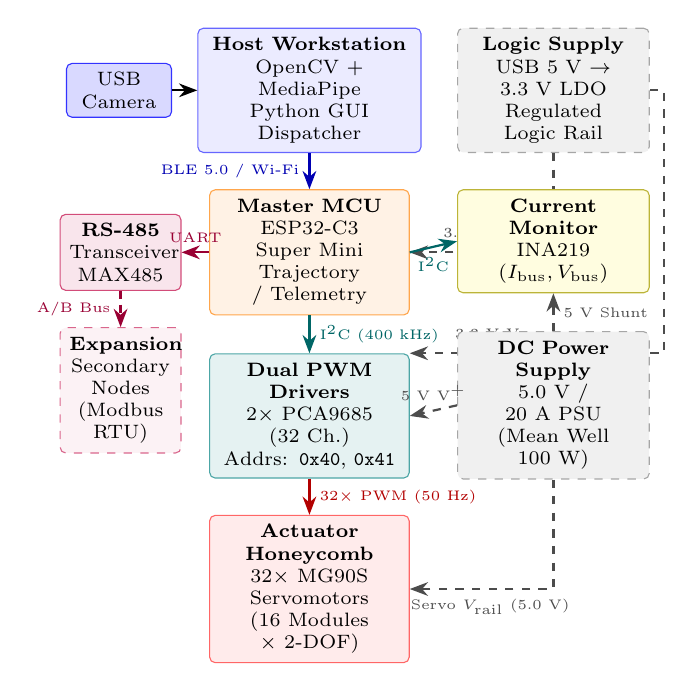
\begin{tikzpicture}[
			>=Stealth,
			node distance=0.32cm and 0.30cm,
			box/.style={draw, rectangle, rounded corners=2pt, minimum height=0.52cm, text centered, font=\scriptsize},
			host/.style={box, fill=blue!8, draw=blue!60, text width=2.6cm},
			mcu/.style={box, fill=orange!10, draw=orange!70, text width=2.3cm},
			driver/.style={box, fill=teal!10, draw=teal!70, text width=2.3cm},
			actuator/.style={box, fill=red!8, draw=red!60, text width=2.3cm},
			sensor/.style={box, fill=yellow!12, draw=yellow!70!black, text width=2.2cm},
			pwr/.style={box, fill=gray!12, draw=gray!70, dashed, text width=2.2cm},
			wire/.style={->, thick},
			sig/.style={wire, blue!70!black},
			i2c/.style={wire, teal!80!black},
			pwm/.style={wire, red!70!black},
			pwrline/.style={wire, dashed, gray!60!black}
			]
			% High-level Perception & Host
			\node[host] (pc) {\textbf{Host Workstation}\\OpenCV + MediaPipe\\Python GUI Dispatcher};
			\node[box, fill=blue!15, draw=blue!80, left=0.32cm of pc, text width=1.1cm] (cam) {USB Camera};
			\draw[wire] (cam) -- (pc);
			
			% 3.3 V Logic Regulator / Rail
			\node[pwr, right=0.45cm of pc] (ldo) {\textbf{Logic Supply}\\USB 5~V $\to$ 3.3~V LDO\\Regulated Logic Rail};
			
			% Master MCU
			\node[mcu, below=0.46cm of pc] (esp) {\textbf{Master MCU}\\ESP32-C3 Super Mini\\Trajectory / Telemetry};
			\draw[sig] (pc) -- node[left, font=\tiny] {BLE 5.0 / Wi-Fi} (esp);
			\draw[pwrline] (ldo.south) |- node[above, pos=0.72, font=\tiny] {3.3~V $\text{V}_{\text{DD}}$} (esp.east);
			
			% Sensors & Expansion Bus
			\node[sensor, below=0.46cm of ldo] (ina) {\textbf{Current Monitor}\\INA219 ($I_{\text{bus}}, V_{\text{bus}}$)};
			\draw[i2c] (esp.east) -- node[below, font=\tiny] {I$^2$C} (ina.west);
			
			\node[box, fill=purple!10, draw=purple!70, left=0.35cm of esp, text width=1.3cm] (rs485) {\textbf{RS-485}\\Transceiver\\MAX485};
			\draw[wire, purple!80!black] (esp) -- node[above, font=\tiny] {UART} (rs485);
			
			% Future multi-node expansion target
			\node[box, fill=purple!5, draw=purple!60, dashed, below=0.46cm of rs485, text width=1.3cm] (modbus) {\textbf{Expansion}\\Secondary Nodes\\(Modbus RTU)};
			\draw[wire, densely dashed, purple!80!black] (rs485) -- node[left, font=\tiny] {A/B Bus} (modbus);
			
			% PWM Drivers
			\node[driver, below=0.48cm of esp] (pca) {\textbf{Dual PWM Drivers}\\$2\times$ PCA9685 (32 Ch.)\\Addrs: \texttt{0x40}, \texttt{0x41}};
			\draw[i2c] (esp) -- node[right, font=\tiny] {I$^2$C (400~kHz)} (pca);
			\draw[pwrline] (ldo.east) -- ++(0.18,0) |- node[above, pos=0.82, font=\tiny] {3.3~V $\text{V}_{\text{CC}}$} (pca.north east);
			
			% Actuators
			\node[actuator, below=0.46cm of pca] (servos) {\textbf{Actuator Honeycomb}\\$32\times$ MG90S Servomotors\\(16 Modules $\times$ 2-DOF)};
			\draw[pwm] (pca) -- node[right, font=\tiny] {32$\times$ PWM (50~Hz)} (servos);
			
			% Power Supply
			\node[pwr, below=0.48cm of ina] (psu) {\textbf{DC Power Supply}\\5.0~V / 20~A PSU\\(Mean Well 100~W)};
			\draw[pwrline] (psu.north) -- node[right, font=\tiny] {5~V Shunt} (ina.south);
			\draw[pwrline] (psu.west) -- node[above, font=\tiny] {5~V $\text{V}^+$} (pca.east);
			\draw[pwrline] (psu.south) |- node[below, pos=0.72, font=\tiny] {Servo $V_{\text{rail}}$ (5.0~V)} (servos.east);
		\end{tikzpicture}
		\caption{Hierarchical hardware, power, and signal architecture of the SOFIA robotic surface, illustrating 3.3~V logic regulation, 5.0~V high-side current monitoring, dual I$^2$C PWM distribution, and provisioned RS-485 Modbus expansion.}
		\label{fig:block_architecture}
	\end{figure}
	
	\subsection{Mechanical Design and Assembly}
	
	As shown in Fig.~\ref{fig:sofia_mechanical_design}, the 2-DOF SOFIA module integrates a structural base, a central gimbal support mechanism, and a hexagonal upper facet cover. The 3D assembly (Fig.~\ref{fig:sofia_mechanical_design}a) and exploded view (Fig.~\ref{fig:sofia_mechanical_design}b) illustrate the orthogonal mounting of the two MG90S servomotors and M3 fastener alignment.
	
	\begin{figure}[!t]
		\centering
		\subfloat[3D assembly.]{
			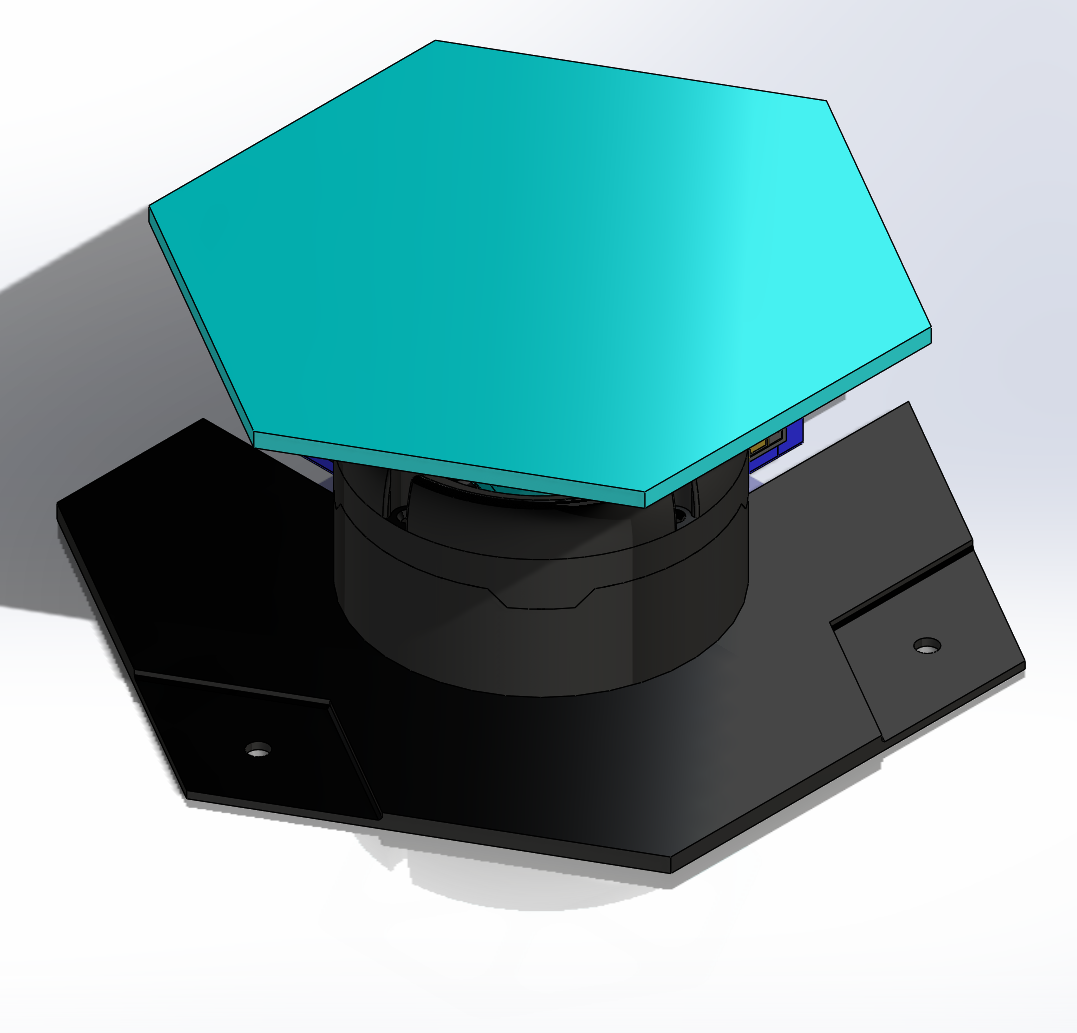
\includegraphics[width=0.47\columnwidth,keepaspectratio]{figures/sofia_solid.png}
		}
		\hfill
		\subfloat[Exploded view.]{
			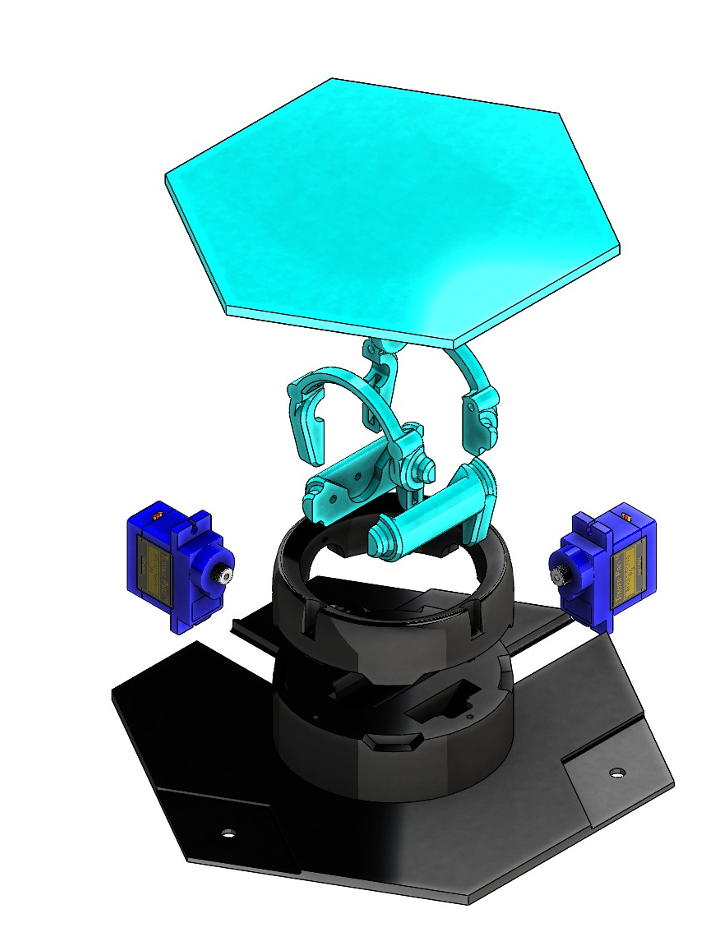
\includegraphics[width=0.47\columnwidth,keepaspectratio]{figures/sofia_exploded.png}
		}
		\caption{SOFIA module 2-DOF CAD assembly and exploded structural views.}
		\label{fig:sofia_mechanical_design}
	\end{figure}
	
	
	\subsection{Kinematic Modeling of the 2-DOF Robotic Unit}
	\label{sec:module_kinematics}
	
	\linelabel{ln:kin-intro}Each modular unit $m_i$ ($i \in \{1, \dots, 16\}$) of the SOFIA kinetic surface comprises a 2-DOF pan-tilt mechanism actuated by two orthogonal MG90S servomotors with joint angular coordinates $\mathbf{q} = [q_1, q_2]^\top$. In single-axis characterization experiments, $\theta \equiv q_j$ ($j \in \{1, 2\}$) denotes the coordinate of the actuator under test.
	
	To establish the analytical forward kinematics, a kinematic tree of reference frames is defined by the chain of coordinate origins $o_0 \prec o_1 \prec o_2 \prec o_3$ (global surface datum $o_0$, module mounting centroid $o_1$ at $\mathbf{r}_{0,2}^{(i)} \in \mathbb{R}^3$, intermediate pitch gimbal $o_2$ rotated by $q_1$ around local $X$, and hexagonal facet end-effector $o_3$ rotated by $q_2$ around intermediate $Y$).
	
	The composite orientation matrix $\mathbf{R}_{1,3}(q_1, q_2) \in \mathrm{SO}(3)$ of the facet relative to the module base is given by successive elementary rotations $\mathbf{R}_{1,3} = \mathbf{R}_x(q_1)\mathbf{R}_y(q_2)$ in \eqref{eq:composite_rot}:
	\begin{align}
		\mathbf{R}_x(q_1) &= \begin{bmatrix} 1 & 0 & 0 \\ 0 & c_1 & -s_1 \\ 0 & s_1 & c_1 \end{bmatrix}, \label{eq:elementary_rot_x} \\
		\mathbf{R}_y(q_2) &= \begin{bmatrix} c_2 & 0 & s_2 \\ 0 & 1 & 0 \\ -s_2 & 0 & c_2 \end{bmatrix}, \label{eq:elementary_rot_y} \\
		\mathbf{R}_{1,3} &= \begin{bmatrix}
			c_2 & 0 & s_2 \\
			s_1 s_2 & c_1 & -s_1 c_2 \\
			-c_1 s_2 & s_1 & c_1 c_2
		\end{bmatrix}, \label{eq:composite_rot}
	\end{align}
	where $s_j \equiv \sin q_j$ and $c_j \equiv \cos q_j$ ($j \in \{1, 2\}$) denote compact trigonometric shorthands.
	
	Defining the nominal unit normal vector of the facet in its rest frame as $\hat{\mathbf{n}}_0 = [0, 0, 1]^\top$, the instantaneous surface normal vector $\hat{\mathbf{r}}_{2,3}^{(i)}$ expressed in module base coordinates and its closed-form inverse kinematics for target pointing direction $\hat{\mathbf{u}} = [u_x, u_y, u_z]^\top = (\mathbf{p} - \mathbf{r}_{0,2}^{(i)}) / \lVert \mathbf{p} - \mathbf{r}_{0,2}^{(i)} \rVert$ are:
	\begin{align}
		\hat{\mathbf{r}}_{2,3}^{(i)} &= \mathbf{R}_{1,3} \hat{\mathbf{n}}_0 = \begin{bmatrix} s_2 \\ -s_1 c_2 \\ c_1 c_2 \end{bmatrix}, \label{eq:facet_normal} \\
		q_2 &= \arcsin(u_x), \quad q_1 = \operatorname{atan2}(-u_y, u_z), \label{eq:ik_closed_form}
	\end{align}
	\linelabel{ln:r3-8-map}where $q_j \in [-30^\circ, +30^\circ]$ ($j \in \{1, 2\}$) denotes the zero-centered kinematic model angle in degrees, which maps to the physical servo command angle $q_j^{\text{servo}}$ via the affine transformation:
	\begin{equation}
		q_j^{\text{servo}} = 90^\circ + q_j, \quad q_j \in [-30^\circ, +30^\circ] \iff q_j^{\text{servo}} \in [60^\circ, 120^\circ],
		\label{eq:servo_mapping}
	\end{equation}
	with $q_j = 0^\circ$ ($q_j^{\text{servo}} = 90^\circ$) corresponding to the horizontal neutral home posture, as evaluated in Algorithm~\ref{alg:sofia_ik}. In the host GUI, raw normalized wrist displacements $q_{j,\text{raw}} \in [-90^\circ, +90^\circ]$ are linearly scaled by $1/3$ into $q_j = (30^\circ / 90^\circ)q_{j,\text{raw}} \in [-30^\circ, +30^\circ]$ before applying \eqref{eq:servo_mapping}. Note that the $[19.3^\circ, 70.2^\circ]$ range ($\Delta q_{\max} = 50.9^\circ$) recorded during preliminary bench testing (Table~\ref{tab:compliance}) reflects the uncentered mechanical travel prior to aligning the servo horn at $q_j^{\text{servo}} = 90^\circ$.
	
	
	\begin{algorithm}[!t]
		\caption{SOFIA Module Inverse Kinematics}
		\label{alg:sofia_ik}
		\footnotesize
		\begin{algorithmic}[1]
			\Require Module origin $\mathbf{r}_{0,2}^{(i)}$, target $\mathbf{p}$, joint limits
			\Ensure Joint angles $q_1,q_2$
			\State $\mathbf{d} \gets \mathbf{p}-\mathbf{r}_{0,2}^{(i)}$
			\State $\mathbf{u} \gets \mathbf{d}/\|\mathbf{d}\|$
			\State $q_2 \gets \arcsin(u_x)$
			\State $q_1 \gets \operatorname{atan2}(-u_y,u_z)$
			\State $q_1 \gets \operatorname{clip}(q_1,q_{1,\min},q_{1,\max})$
			\State $q_2 \gets \operatorname{clip}(q_2,q_{2,\min},q_{2,\max})$
			\State \Return $q_1,q_2$
		\end{algorithmic}
	\end{algorithm}
	
	
	\subsection{Computer Vision Tracking and Dynamic Gesture Pipeline}
	\label{sec:vision_pipeline}
	
	\linelabel{ln:vis}The perception layer is developed using Python 3.11 with MediaPipe Tasks and OpenCV in a modular, low-latency pipeline. Real-time tracking uses \linelabel{ln:vis-mp}Google MediaPipe Landmarker models in video streaming mode, extracting 33 body landmarks and two sets of 21 3D hand coordinates $(x,y,z)$ with millisecond timestamps, sustaining 30~FPS on standard CPUs without dedicated GPU acceleration.
	
	Finger extension is evaluated using distal-to-wrist 3D Euclidean distances normalized by palm scale $\lVert \mathbf{p}_{\text{wrist}}-\mathbf{p}_{\text{MCP}}\rVert$, reducing perspective and depth-related distortions.
	
	The \textit{GestureDetector} arbitrates static and dynamic gestures using temporal and priority rules. The wave\linelabel{ln:vis-es1} gesture is detected when at least three consecutive direction reversals occur in the MCP joint's lateral coordinate (landmark 9), with peak-to-peak amplitude above $0.05$ normalized units. The two-handed rock--paper--scissors gesture uses a finite-state machine with contact and release thresholds of $d_{\text{contact}}<0.17$ and $d_{\text{release}}>0.20$\linelabel{ln:vis-es2}. Temporal hysteresis reduces false triggers during transitions. Static commands include two-handed heart gestures, open palms, victory signs, and closed fists.
	
	The PySide6 interface integrates live video, gesture telemetry, FPS/latency badges, manual sliders, and channel toggles (Fig.~\ref{fig:sofia_gui}), locking joint angles to $[60^\circ, 120^\circ]$ and suspending tracking during active routines.
	
	\begin{figure}[!t]
		\centering
		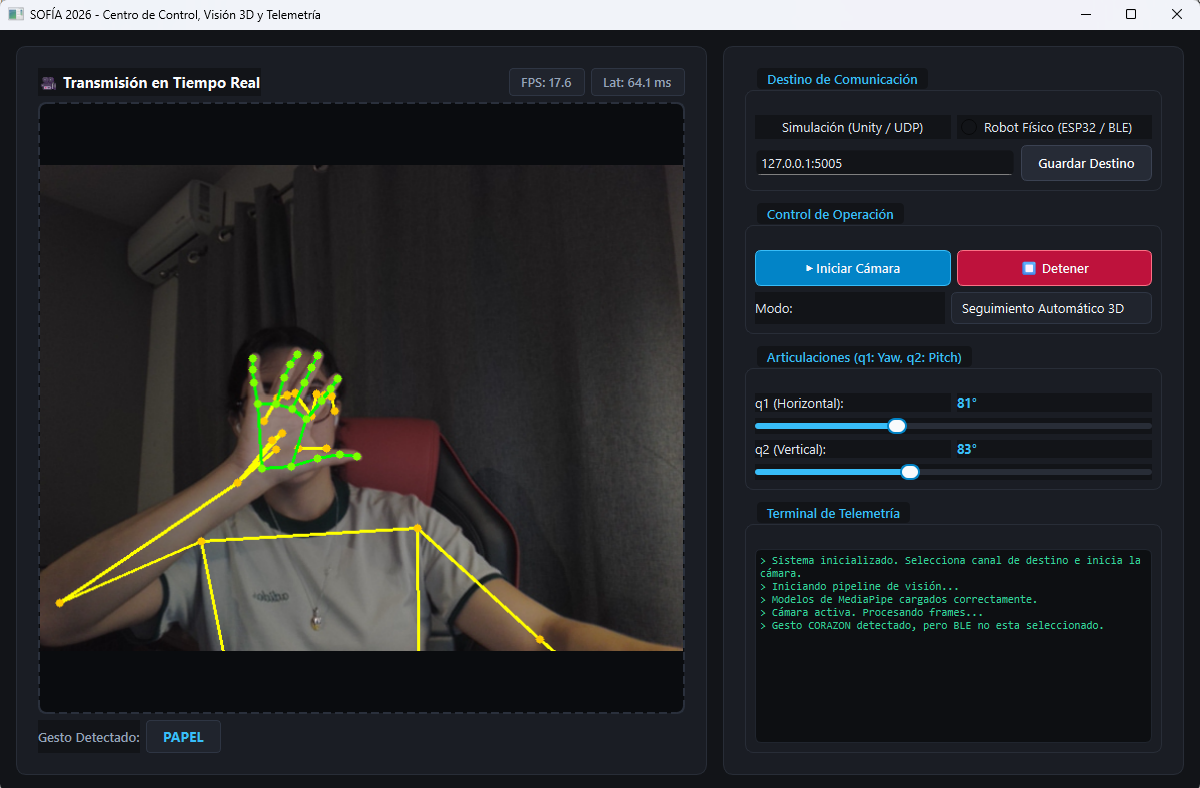
\includegraphics[width=0.68\columnwidth,height=1.9cm,keepaspectratio]{figures/sofia_gui.png}
		\caption{SOFIA graphical interface for vision monitoring and robot control.}
		\label{fig:sofia_gui}
	\end{figure}
	
	\begin{figure*}[!t]
		\centering
		\subfloat[$t_1$: target left-up.]{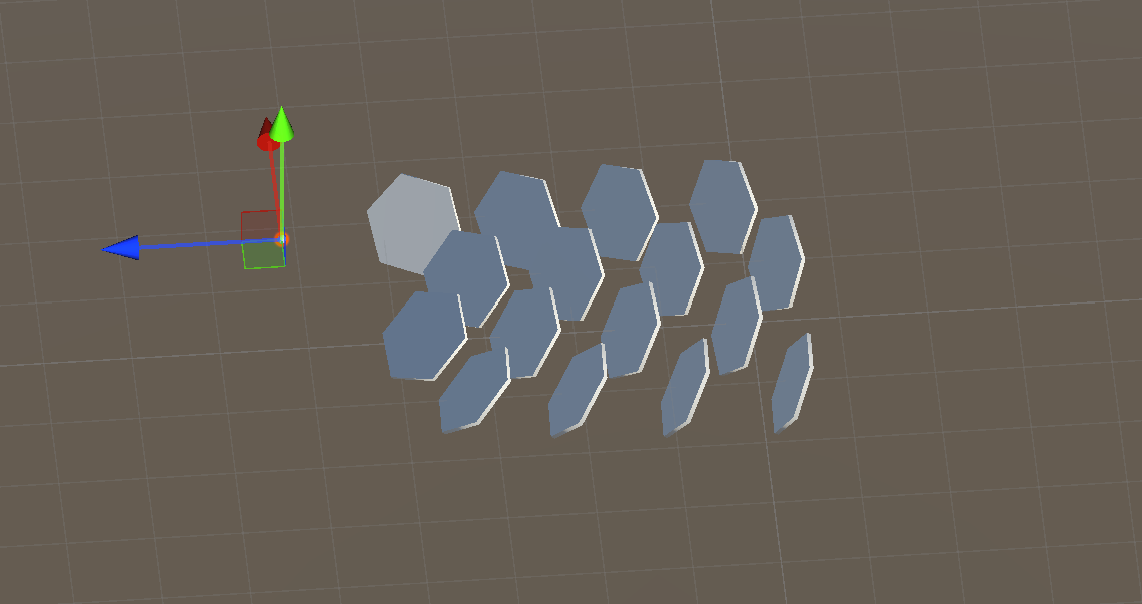
\includegraphics[width=0.31\textwidth,keepaspectratio]{figures/fig_sim_1.png}}\hfill
		\subfloat[$t_2$: sweep center.]{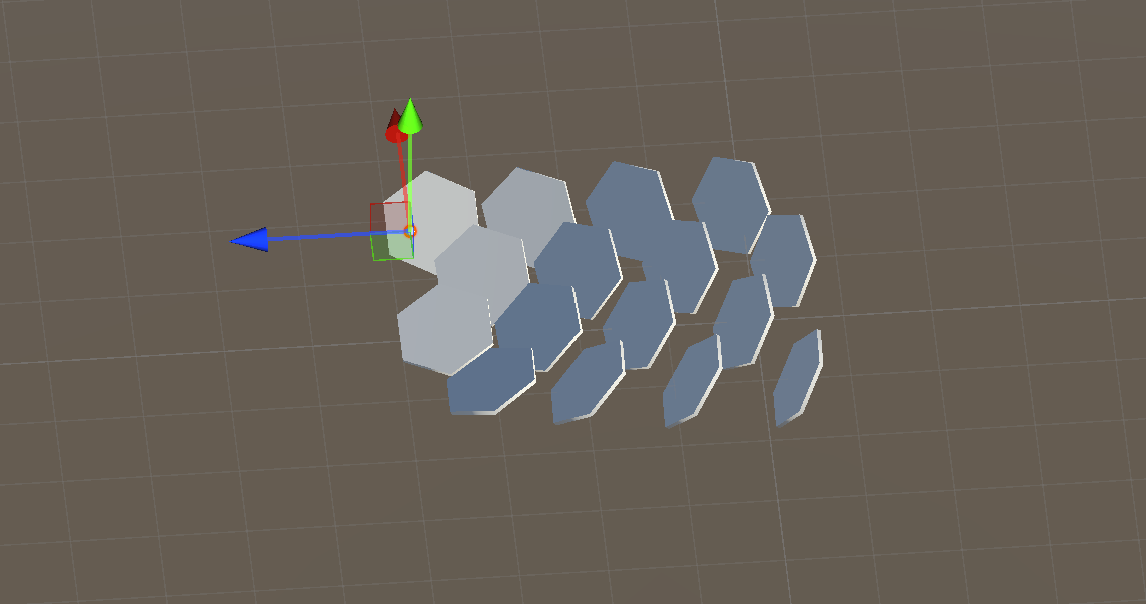
\includegraphics[width=0.31\textwidth,keepaspectratio]{figures/fig_sim_2.png}}\hfill
		\subfloat[$t_3$: target right-up.]{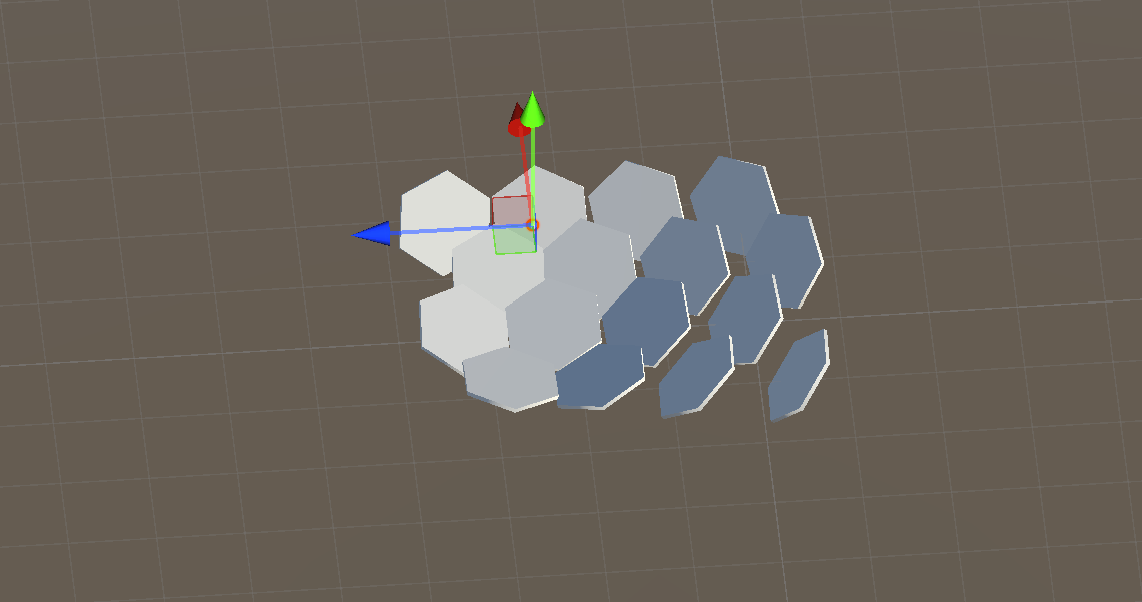
\includegraphics[width=0.31\textwidth,keepaspectratio]{figures/fig_sim_3.png}}\\[4pt]
		\subfloat[$t_4$: lower-right tilt.]{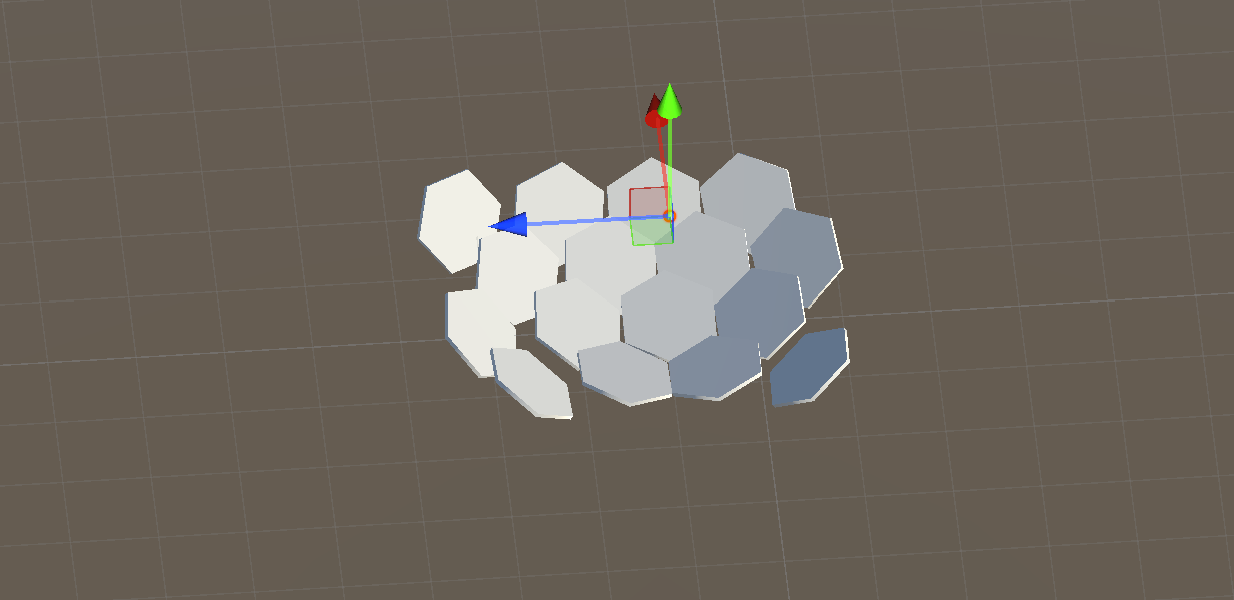
\includegraphics[width=0.31\textwidth,keepaspectratio]{figures/fig_sim_4.png}}\hfill
		\subfloat[$t_5$: lower-center tilt.]{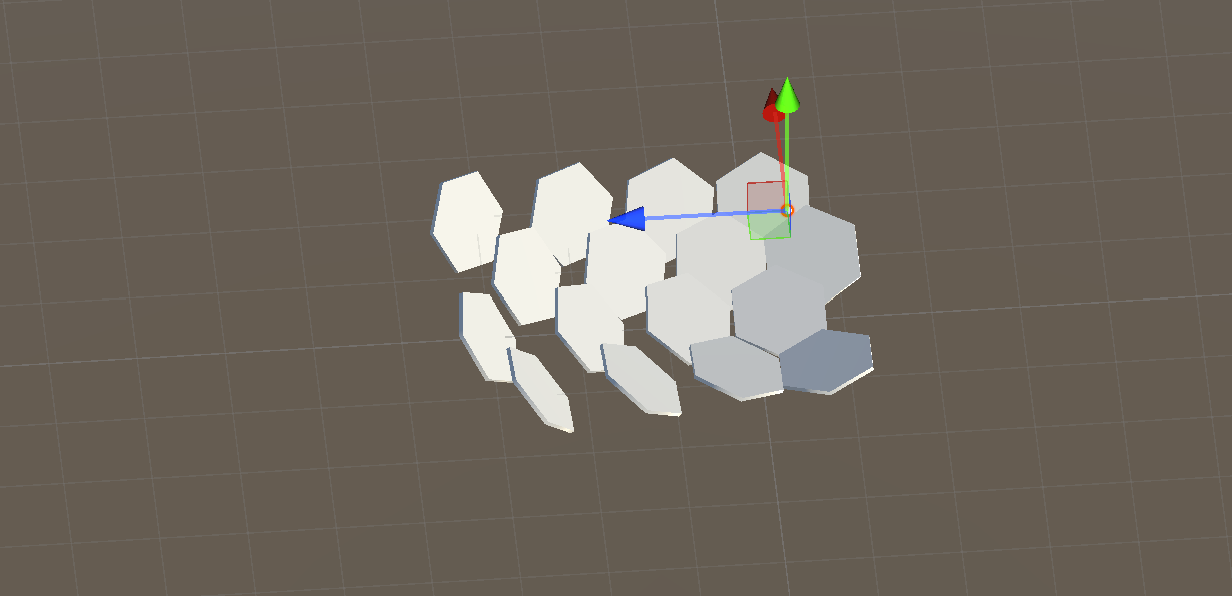
\includegraphics[width=0.31\textwidth,keepaspectratio]{figures/fig_sim_5.png}}\hfill
		\subfloat[$t_6$: lower-left return.]{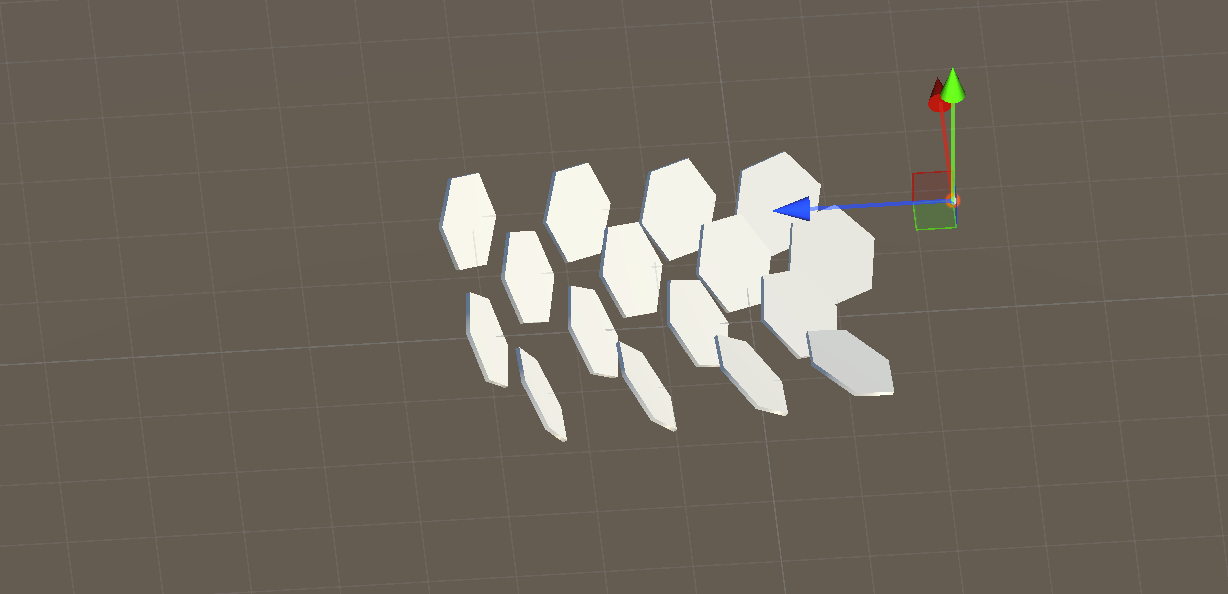
\includegraphics[width=0.31\textwidth,keepaspectratio]{figures/fig_sim_6.png}}
		\caption{Representative frames of the SOFIA 16-module kinematic tracking simulation across six target waypoints $\mathbf{p}(t_1)\text{--}\mathbf{p}(t_6)$, showing the reference coordinate triad $(X,Y,Z)$ and coordinated facet reorientation.}
		\label{fig:sofia_simulation}
	\end{figure*}
	
	\linelabel{ln:r3-10-smooth}The control strategy distinguishes between continuous joint tracking and discrete choreographic routines. To eliminate high-frequency landmark jitter and abrupt servo steps during continuous tracking, a two-stage smoothing and rate-limiting pipeline is implemented: first, 3D MediaPipe coordinates $\mathbf{p}_k$ are filtered in \texttt{LandmarkSmoother} using an exponential moving average (EMA), $\hat{\mathbf{p}}_k = \alpha \mathbf{p}_k + (1 - \alpha)\hat{\mathbf{p}}_{k-1}$ with $\alpha = 0.35$; second, the BLE dispatcher enforces a $5\text{ Hz}$ ($\Delta t_{\min} = 200\text{ ms}$) transmission rate limiter with single-slot queue replacement (\texttt{\_ultimo\_ang}), discarding stale intermediate setpoints and bounding maximum slewing velocity to $\le 150^\circ/\text{s}$. For static gestures (\texttt{CORAZON}, \texttt{TIJERA}, \texttt{ROCA}, \texttt{PAPEL}), \texttt{PostureTrigger} requires a $0.6\text{ s}$ continuous hold with wrist angular variance $\le 12^\circ$ and a $1.0\text{ s}$ post-trigger cooldown, following the posture-validation state machine in Fig.~\ref{fig:maquina_estado_sofia}.
	
	\begin{figure}[!t]
		\centering
		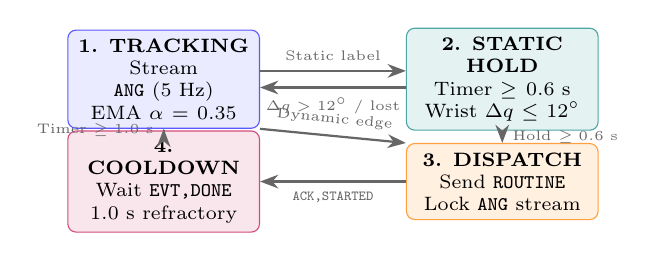
\begin{tikzpicture}[
			>=Stealth,
			state/.style={draw, rectangle, rounded corners=3pt, minimum height=0.55cm, text width=2.2cm, align=center, font=\scriptsize},
			idle/.style={state, fill=blue!8, draw=blue!65},
			hold/.style={state, fill=teal!10, draw=teal!70},
			trig/.style={state, fill=orange!12, draw=orange!75},
			cool/.style={state, fill=purple!10, draw=purple!70},
			trans/.style={->, thick, gray!80!black, font=\tiny}
			]
			\node[idle] (idle) at (0, 0) {\textbf{1. TRACKING}\\Stream \texttt{ANG} ($5\text{ Hz}$)\\EMA $\alpha=0.35$};
			\node[hold] (hold) at (4.3, 0) {\textbf{2. STATIC HOLD}\\Timer $\ge 0.6\text{ s}$\\Wrist $\Delta q \le 12^\circ$};
			\node[trig] (trig) at (4.3, -1.30) {\textbf{3. DISPATCH}\\Send \texttt{ROUTINE}\\Lock \texttt{ANG} stream};
			\node[cool] (cool) at (0, -1.30) {\textbf{4. COOLDOWN}\\Wait \texttt{EVT,DONE}\\$1.0\text{ s}$ refractory};
			
			\draw[trans] ([yshift=3pt]idle.east) -- node[above] {Static label} ([yshift=3pt]hold.west);
			\draw[trans] ([yshift=-3pt]hold.west) -- node[below] {$\Delta q > 12^\circ$ / lost} ([yshift=-3pt]idle.east);
			\draw[trans] (hold.south) -- node[right] {Hold $\ge 0.6\text{ s}$} (trig.north);
			\draw[trans] (idle.south east) -- node[above, sloped] {Dynamic edge} (trig.north west);
			\draw[trans] (trig.west) -- node[below] {\texttt{ACK,STARTED}} (cool.east);
			\draw[trans] (cool.north) -- node[left] {Timer $\ge 1.0\text{ s}$} (idle.south);
		\end{tikzpicture}
		\caption{Finite-state machine governing posture recognition, validation, and motion command execution in \texttt{PostureTrigger}.}
		\label{fig:maquina_estado_sofia}
	\end{figure}
	
	\subsection{Firmware Architecture, Electronic Interconnection, and Integration Lessons}
	\label{sec:hardware_stage}
	
	\linelabel{ln:r3-10-fsm}On the embedded side (\texttt{modulo\_sofia.ino}), the ESP32-C3 runs a non-blocking finite-state machine (Fig.~\ref{fig:firmware_fsm}) decoupled from BLE GATT interrupt callbacks via an 8-slot FreeRTOS message queue (\texttt{colaTramas}). Upon boot, the controller initializes I$^2$C ($400\text{ kHz}$ on SDA~8 / SCL~9), verifies PCA9685 acknowledgment at \texttt{0x40} (\texttt{pcaDisponible}), and enters the \textbf{IDLE / HOME} state. Incoming \texttt{\$SEQ,ANG,q1,q2\#} frames transition the unit to \textbf{TRACKING}, applying \eqref{eq:servo_mapping} and returning \texttt{\$SEQ,ACK,OK,q1,q2\#}. When a \texttt{\$SEQ,ROUTINE,<NAME>\#} frame arrives, the FSM transitions to \textbf{ROUTINE}, locking out tracking commands (\texttt{NACK,ERR\_04}), returning \texttt{\$SEQ,ACK,STARTED,<NAME>\#}, and stepping through the stored waypoint table using non-blocking \texttt{millis()} timers ($300\text{--}500\text{ ms}$ per step). Upon completing the final repetition, the firmware emits \texttt{\$SEQ,EVT,DONE,<NAME>\#} and returns to \textbf{IDLE}, re-enabling tracking. If an I$^2$C fault occurs (\texttt{ERR\_05}), a \texttt{STOP} command is received, or the BLE client disconnects (\texttt{onDisconnect}), the FSM enters \textbf{FAULT / SAFE HOME}, driving both servos to $(90^\circ, 90^\circ)$ (or cutting PWM via full-off bit \texttt{4096}) and restarting BLE advertising.
	
	\begin{figure}[!t]
		\centering
		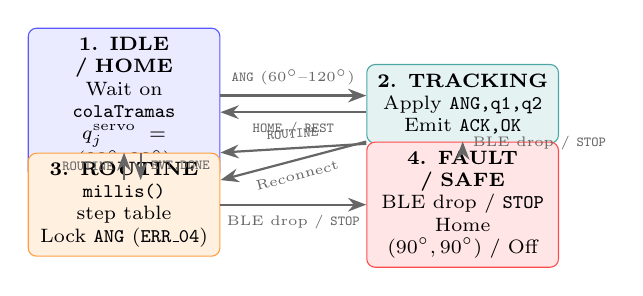
\begin{tikzpicture}[
			>=Stealth,
			state/.style={draw, rectangle, rounded corners=3pt, minimum height=0.55cm, text width=2.2cm, align=center, font=\scriptsize},
			idle/.style={state, fill=blue!8, draw=blue!65},
			trk/.style={state, fill=teal!10, draw=teal!70},
			rot/.style={state, fill=orange!12, draw=orange!75},
			flt/.style={state, fill=red!10, draw=red!70},
			trans/.style={->, thick, gray!80!black, font=\tiny}
			]
			\node[idle] (idle) at (0, 0) {\textbf{1. IDLE / HOME}\\Wait on \texttt{colaTramas}\\$q_j^{\text{servo}} = (90^\circ, 90^\circ)$};
			\node[trk] (trk) at (4.3, 0) {\textbf{2. TRACKING}\\Apply \texttt{ANG,q1,q2}\\Emit \texttt{ACK,OK}};
			\node[rot] (rot) at (0, -1.28) {\textbf{3. ROUTINE}\\\texttt{millis()} step table\\Lock \texttt{ANG} (\texttt{ERR\_04})};
			\node[flt] (flt) at (4.3, -1.28) {\textbf{4. FAULT / SAFE}\\BLE drop / \texttt{STOP}\\Home $(90^\circ,90^\circ)$ / Off};
			
			\draw[trans] ([yshift=3pt]idle.east) -- node[above] {\texttt{ANG} ($60^\circ\text{--}120^\circ$)} ([yshift=3pt]trk.west);
			\draw[trans] ([yshift=-3pt]trk.west) -- node[below] {\texttt{HOME} / \texttt{REST}} ([yshift=-3pt]idle.east);
			\draw[trans] (idle.south) -- node[left] {\texttt{ROUTINE}} (rot.north);
			\draw[trans] (trk.south west) -- node[above, sloped] {\texttt{ROUTINE}} (rot.north east);
			\draw[trans] ([xshift=6pt]rot.north) -- node[right] {\texttt{EVT,DONE}} ([xshift=6pt]idle.south);
			\draw[trans] (trk.south) -- node[right] {BLE drop / \texttt{STOP}} (flt.north);
			\draw[trans] (rot.east) -- node[below] {BLE drop / \texttt{STOP}} (flt.west);
			\draw[trans] (flt.north west) -- node[below, sloped] {Reconnect} (idle.south east);
		\end{tikzpicture}
		\caption{ESP32-C3 firmware finite-state machine (\texttt{modulo\_sofia.ino}) governing mutual exclusion between tracking, choreographic routines, and fail-safe recovery.}
		\label{fig:firmware_fsm}
	\end{figure}
	
	In the current\linelabel{ln:hwstage}\linelabel{ln:r3-10-lessons}\linelabel{ln:r4-3-inc} Apply and Build \& Validate stages, system integration proceeded across five sequential increments documented in the project engineering logbook and repository commit history (Table~\ref{tab:integration_increments}), progressing from minimal single-axis PWM actuation to full fault-tolerant vision-to-BLE closed-loop operation on breadboard while the custom 4-layer PCB (Fig.~\ref{fig:sofia_pcb_design}) undergoes fabrication (\linelabel{ln:hw-make}full 32-actuator array assembly on the fabricated PCB constitutes Increment~5). Three critical integration failures directly reshaped the final design: (i) the Trial~1 gear-retainer thermal failure ($64.84^\circ\text{C}$ at $180^\circ$) and mechanical interference between adjacent 3D-printed petals ($\pm 0.4\text{ mm}$ tolerance) prompted restricting the software command workspace to $q_j^{\text{servo}} \in [60^\circ, 120^\circ]$ and enforcing auto-homing on disconnect; (ii) early unframed BLE string writes (\texttt{"SALUDO"}) suffered from silent packet drops and fixed $3\text{ s}$ GUI timers that desynchronized tracking from physical motion, motivating the framed \texttt{\$SEQ,CMD\#} protocol with \texttt{SEQ} deduplication and asynchronous \texttt{EVT,DONE} unlocking; and (iii) executing servo updates inside the BLE callback caused FreeRTOS watchdog resets, which was resolved by decoupling reception and actuation via \texttt{colaTramas}.
	
	\begin{table}[!t]
		\centering
		\caption{Incremental Subsystem Integration and Verification Log}
		\label{tab:integration_increments}
		\scriptsize
		\setlength{\tabcolsep}{2.2pt}
		\renewcommand{\arraystretch}{0.88}
		\begin{tabular}{@{}l c p{2.1cm} p{2.25cm} p{1.4cm}@{}}
			\toprule
			\textbf{Inc.} & \textbf{Date} & \textbf{Integrated Subsystems} & \textbf{Verification \& Outcome} & \textbf{Commit / Log} \\
			\midrule
			\textbf{1} & Sep~28 & Single MG90S + ESP32 + LM35/INA219 bench & Stall heating ($\bar{\beta}_1 = 0.214\,^\circ\text{C/s}$) \& $20\text{ Hz}$ current logs & \texttt{9369fa0} / \texttt{servo\_char.} \\
			\textbf{2} & Oct~05 & 2-DOF module + PCA9685 (\texttt{0x40}) + Unity 16-cell IK & Closed-form IK ($\text{MAE} = 0.00^\circ$ in $\pm 30^\circ$) \& I$^2$C PWM sweep & \texttt{bcc9a52} (\texttt{v0.2.0}) \\
			\textbf{3} & Oct~15 & MediaPipe 3D vision + unframed BLE (\texttt{SALUDO}/\texttt{CORAZON}) & $30\text{ FPS}$ tracking; identified BLE race condition \& $3\text{ s}$ lock bug & \texttt{7a790a3} / \texttt{e0a0c9e} \\
			\textbf{4} & Nov~25 & Framed \texttt{\$SEQ,CMD\#} BLE + FreeRTOS FSM + 7 routines & 7/7 postures, 4/4 NACKs (\texttt{registro\_pruebas\_ciclo.csv}), auto-recovery & \texttt{e95ceaf} (\texttt{v0.4.0}) \\
			\textbf{5} & Pending & 4-layer PCB + $2\times$ PCA9685 + 32 servos + $60\text{ FPS}$ cam & Gerber files in fabrication; array \& optical test scheduled & \texttt{hardware/pcb/} (Pending) \\
			\bottomrule
		\end{tabular}
	\end{table}
	
	
	\begin{figure*}[!t]
		\centering
		\subfloat[Electrical schematic of the ESP32-C3, dual PCA9685, and power distribution tiers.]{
			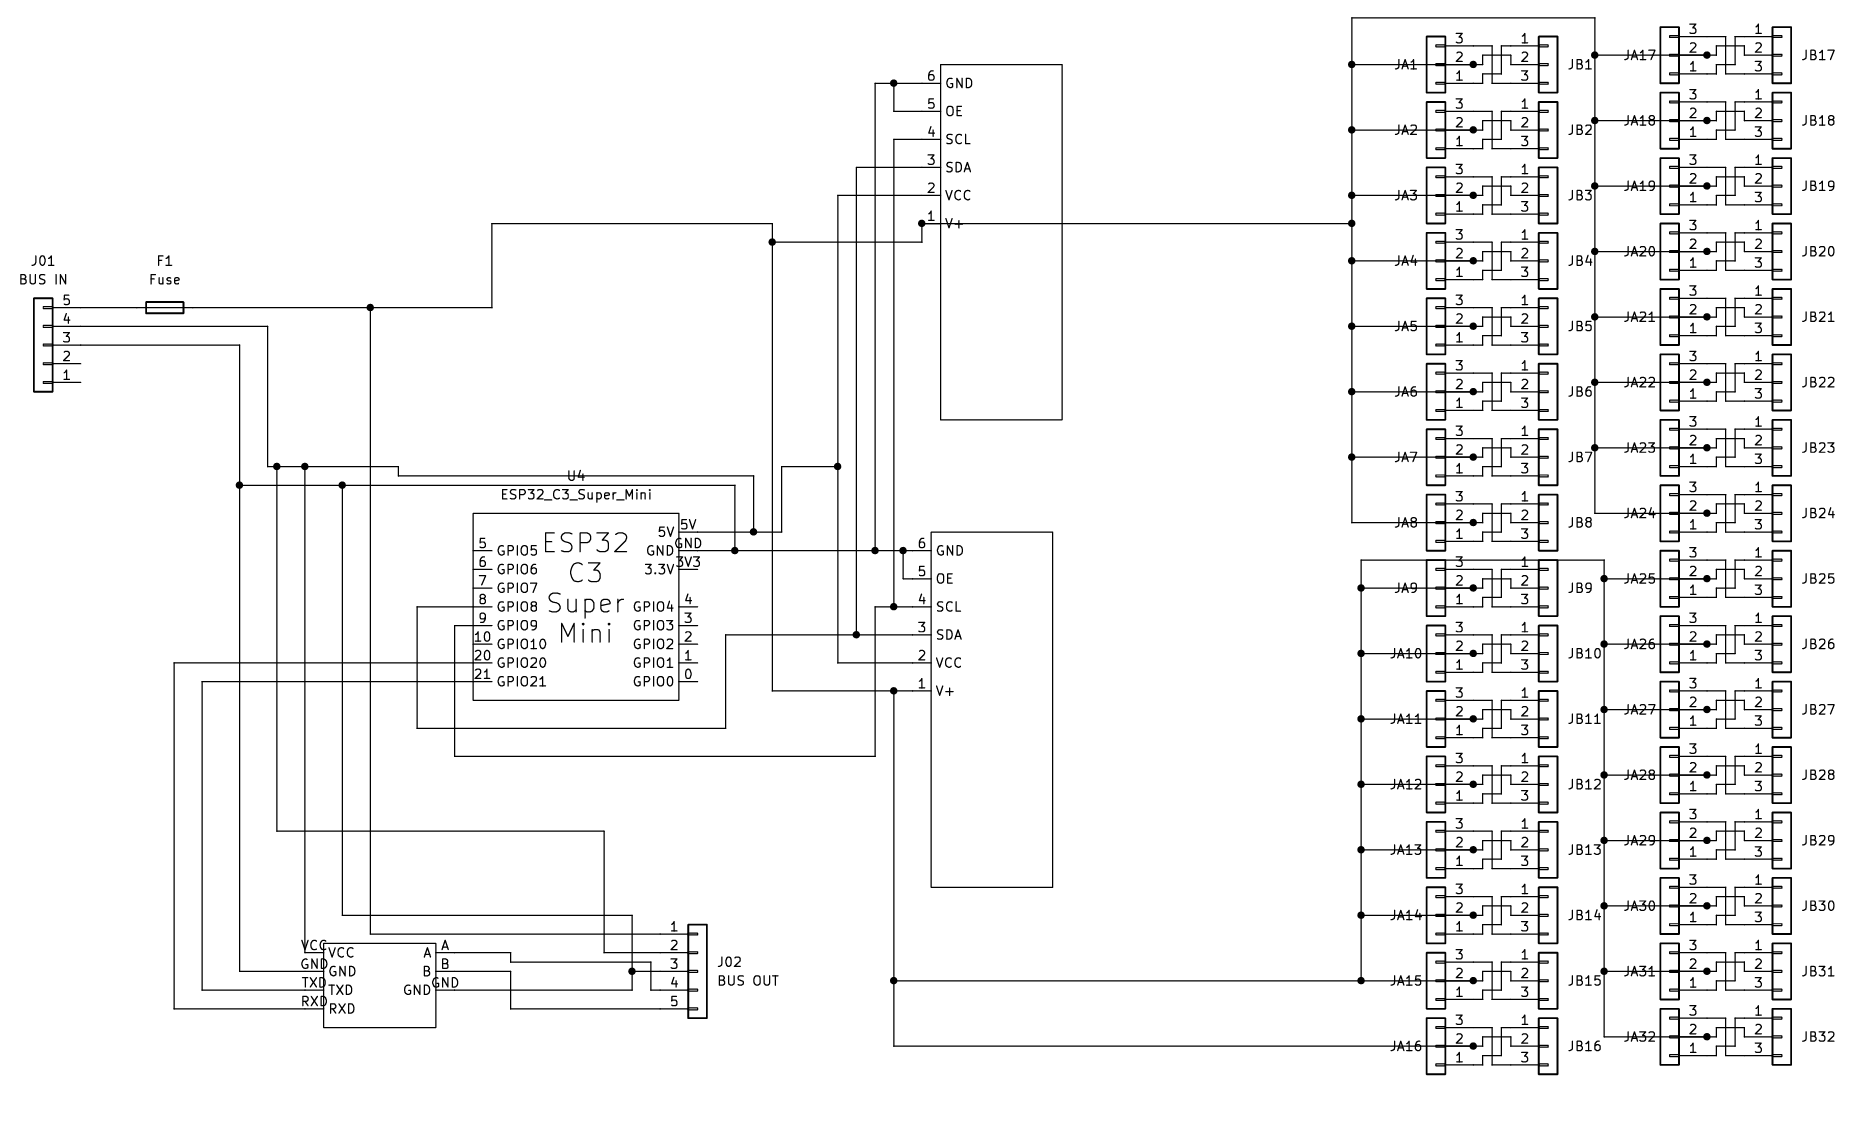
\includegraphics[width=0.52\textwidth,height=3.2cm,keepaspectratio]
			{figures/sofia_schematic.png}
		}\hfill
		\subfloat[Routed PCB layout submitted for fabrication.]{
			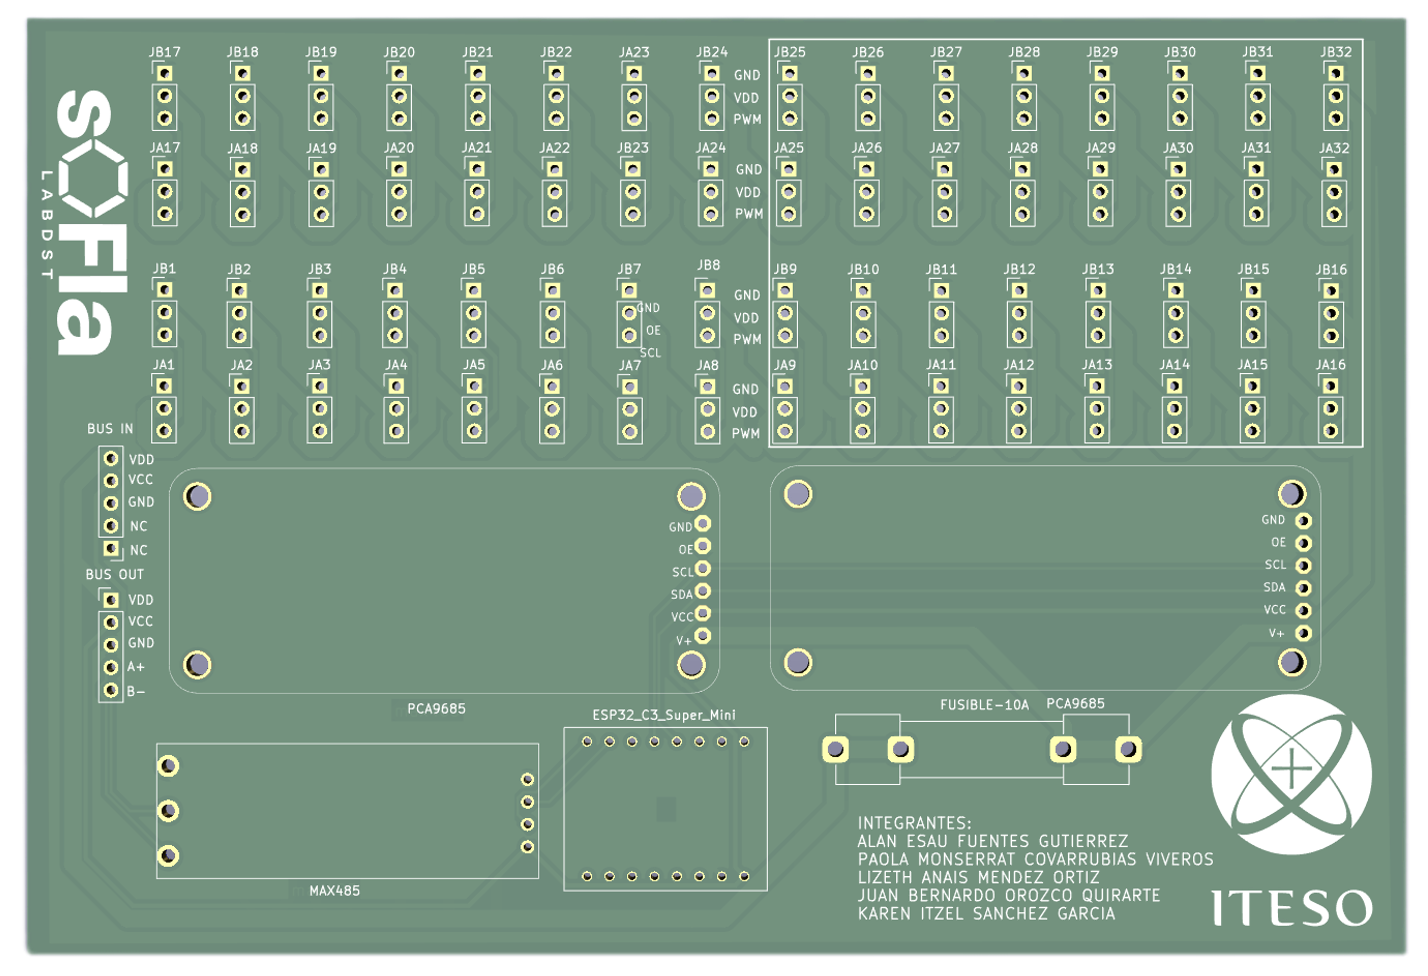
\includegraphics[width=0.43\textwidth,height=3.2cm,keepaspectratio]
			{figures/sofia_pcb_layout.png}
		}
		\caption{SOFIA custom PCB design shown at full two-column width: (a) electrical schematic and
			(b) layout submitted for fabrication.}
		\label{fig:sofia_pcb_design}
	\end{figure*}
	
	\begin{figure*}[!t]
		\centering
		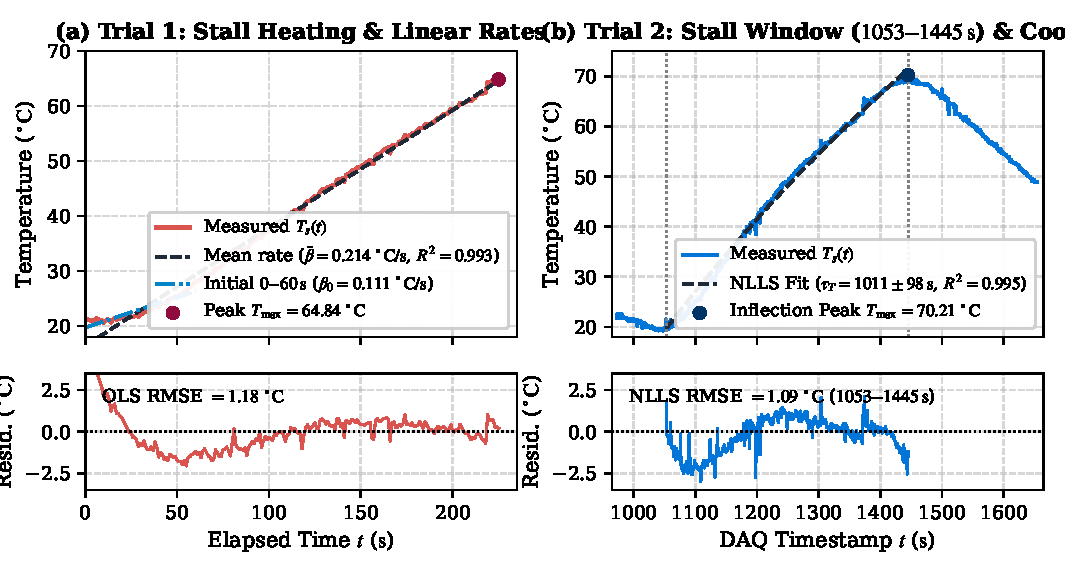
\includegraphics[width=0.90\textwidth,height=3.4cm,keepaspectratio]{figures/fig_thermal_response}
		\caption{Experimental thermal characterization of the MG90S servomotor under persistent stall ($1\text{ Hz}$ LM35 telemetry) with bottom residual panels: (a) Trial~1 continuous heating to $64.84^\circ\text{C}$; and (b) Trial~2 extended stall window ($t_{\text{DAQ}} \in [1053.1, 1445.1]\text{ s}$) with descriptive NLLS fit and subsequent cooling.}
		\label{fig:thermal_response}
	\end{figure*}
	
	\begin{figure*}[!t]
		\centering
		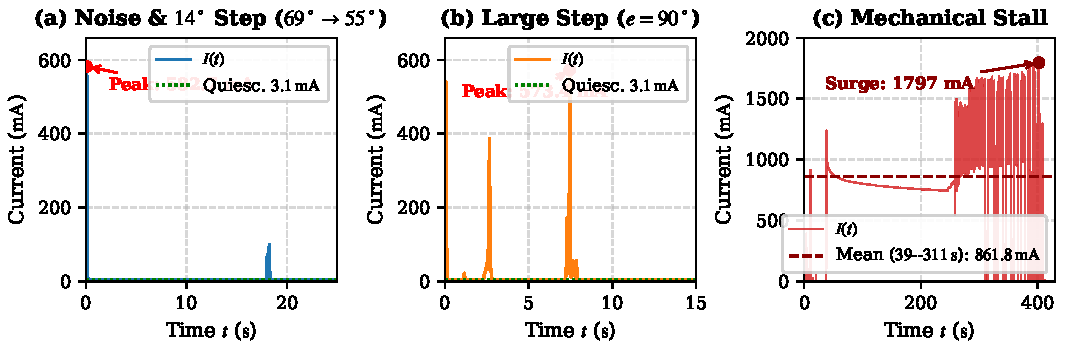
\includegraphics[width=0.92\textwidth,height=2.8cm,keepaspectratio]{figures/fig_current_characterization}
		\caption{Experimental supply current $I(t)$ of the MG90S actuator at $20\text{ Hz}$ on the $5.0\text{ V}$ bus: (a) small step references (\texttt{datos\_5grados.csv}); (b) manual potentiometer sweeps (\texttt{datos\_901.csv}); and (c) persistent mechanical stall (\texttt{datos\_CHIDOS\_DE\_FORZADO.csv}). Quantitative metrics are reported in Section~\ref{sec:thermal_experiment}.}
		\label{fig:characterization_6panels}
		\label{fig:current_characterization}
	\end{figure*}
	
	The \texttt{SofiaCommDispatcher} architecture decouples kinematic
	generation from transmission channels, routing joint angles $(q_1, q_2)$
	bounded to $[60^\circ, 120^\circ]$ and discrete choreographic commands via
	either a framed bidirectional BLE GATT protocol (Nordic UART Service) to
	the physical ESP32-C3 or UDP datagrams to the virtual simulator
	(Table~\ref{tab:sofia_message_contract}). Over BLE, requests follow the
	delimited structure \texttt{\$<SEQ>,<CMD>,<PARAMS>\#}, where \texttt{<SEQ>}
	is an incremental sequence identifier ($1\text{--}65535$) used for packet
	deduplication. The ESP32-C3 processes incoming frames via a FreeRTOS queue
	and returns asynchronous notifications over the TX characteristic
	(\texttt{6e400003}): \texttt{\$<SEQ>,ACK,<DATA>\#} upon validation,
	\texttt{\$<SEQ>,NACK,ERR\_xx\#} upon syntax or range violations, and
	\texttt{\$<SEQ>,EVT,DONE,<ROUTINE>\#} upon completing a choreographic
	sequence. The host enforces a $200\text{ ms}$ response timeout with up to
	two automatic retries, a $4.0\text{ s}$ keepalive \texttt{PING} heartbeat,
	and non-blocking background auto-reconnection ($2.5\text{ s}$ backoff).
	
	\begin{table}[!t]
		\centering
		\caption{SOFIA Bidirectional Communication Protocol Specification}
		\label{tab:sofia_message_contract}
		\scriptsize
		\setlength{\tabcolsep}{3pt}
		\renewcommand{\arraystretch}{0.88}
		\resizebox{\columnwidth}{!}{%
		\begin{tabular}{@{}lll@{}}
			\toprule
			\textbf{Property} & \textbf{BLE (Physical ESP32-C3)} & \textbf{UDP (Unity Simulation)} \\
			\midrule
			Transport & GATT Write (\texttt{6e400002}) / Notify (\texttt{6e400003}) & UDP Socket (\texttt{127.0.0.1:5005}) \\
			Request frame & \texttt{\$SEQ,ANG,q1,q2\#} / \texttt{\$SEQ,ROUTINE,NAME\#} & \texttt{q1,q2} / \texttt{ROUTINE\_NAME} \\
			Response frame & \texttt{\$SEQ,ACK,...\#} / \texttt{NACK,ERR\_xx} / \texttt{EVT,DONE} & Unidirectional (fire-and-forget) \\
			Flow control & $200\text{ ms}$ timeout, 2 retries, $4.0\text{ s}$ \texttt{PING} & Continuous stream ($\le 30\text{ Hz}$) \\
			Fail-safe & Auto-reconnect ($2.5\text{ s}$); servo HOME $(90^\circ,90^\circ)$ & Local angle clamping $[60^\circ,120^\circ]$ \\
			\bottomrule
		\end{tabular}%
		}
	\end{table}
	
	\subsection{Thermal Protection and Reliability Risk Mitigation}
	\label{sec:risk_mitigation}
	
	Based\linelabel{ln:wd}\linelabel{ln:r3-6-wd} on the worst-case empirical heating rate ($\bar{\beta}_1 = 0.214\,^\circ\text{C/s}$) established in Section~\ref{sec:thermal_modeling} and the unified thermal safety ceiling $T_{\text{safe}} = 60^\circ\text{C}$ (set below the $65^\circ\text{C}$ polymer softening threshold), a two-tier protection architecture compatible with the declared hardware is implemented.
	
	\textit{Command-driven channel saturation and timeout limiting.} Because two rail-level INA219 sensors measure aggregate bank current and cannot isolate individual servo channels—and because normal slewing produces $573\text{--}583\text{ mA}$ inrush peaks that would falsely trip a low current threshold—per-channel thermal protection is enforced in the command layer. First, all angle commands are hard-clamped to $q_j^{\text{servo}} \in [60^\circ, 120^\circ]$ (\linelabel{ln:wd-sat}$q_j \in [-30^\circ, +30^\circ]$, Table~\ref{tab:compliance}) to prevent end-stop mechanical stalls. Second, to cover both static holding and continuous tracking, the $15\text{ s}$ protection window is triggered by sustained near-static error ($|q_{\text{cmd}} - q_{\text{cmd,prev}}| \le 2^\circ$ for $\Delta t > 15\text{ s}$ at $q_j^{\text{servo}} \neq 90^\circ$, bounding worst-case rise to $\Delta T = \bar{\beta}_1 \Delta t \approx 3.2^\circ\text{C}$), or on BLE disconnect, issuing \texttt{STOP} (\texttt{pwm.setPWM(ch, 0, 4096)}) or returning to HOME $(90^\circ, 90^\circ)$ before casing temperature approaches $T_{\text{safe}} = 60^\circ\text{C}$.
	
	\textit{Bank-level overcurrent monitoring.} Complementing command-level limiting, each INA219 sensor (configured with an external $10\text{ m}\Omega$ shunt to expand range from $3.2\text{ A}$ to $16\text{ A}$) monitors a 16-servo PCA9685 bank. To reject $< 100\text{ ms}$ inrush spikes while detecting four simultaneous stalls at rest ($4 \times 861.8\text{ mA} + 12 \times 3.12\text{ mA} = 3.48\text{ A}$), the bank fault threshold is set to $\bar{I}_{\text{bank}} > 3.40\text{ A}$ sustained for $> 2.0\text{ s}$, which detects $\ge 4$ stalled servos at rest and $\ge 2$ stalled servos during active tracking ($2 \times 861.8 + 14 \times 135.4\text{ mA} = 3.62\text{ A}$), de-asserting the PCA9685 \texttt{OE} pin. While command-level clamping, \texttt{STOP} pulse suspension, and disconnect auto-homing are verified in the physical prototype, closed-loop INA219 thermal cut-off testing under active stall remains scheduled for the full array (marked \textit{Pending} in Table~\ref{tab:compliance}\linelabel{ln:wd-torque}).
	
	To address operational failure modes beyond thermal stalls, Table~\ref{tab:risk_matrix} systematically details the comprehensive risk assessment \linelabel{ln:r1-5-pi}(Probability / Impact) across perception, communication, power, and actuator tiers.
	
	\begin{table}[!t]
		\centering
		\caption{System Failure Modes, Operational Risk Assessment (\textnormal{P/I}: Probability / Impact), and Mitigation Strategies}
		\label{tab:risk_matrix}
		\scriptsize
		\setlength{\tabcolsep}{2pt}
		\renewcommand{\arraystretch}{0.88}
		\resizebox{\columnwidth}{!}{%
		\begin{tabular}{@{}p{1.55cm} >{\centering\arraybackslash}p{1.25cm} p{3.0cm} p{2.5cm}@{}}
			\toprule
			\textbf{Failure / Risk} & \textbf{P / I}$^{\mathrm{a}}$ & \textbf{Mitigation Strategy} & \textbf{Verification Method} \\
			\midrule
			\textbf{Actuator Stall} & High / High & Command dwell $\Delta t \le 15\text{ s}$ ($|q_{\text{cmd}} - q_{\text{prev}}| \le 2^\circ$); bank trip $\bar{I}_{\text{bank}} > 3.40\text{ A}$ for $>2\text{ s}$ ($T_{\text{safe}} \le 60^\circ\text{C}$). & Command \texttt{STOP}/HOME verified; thermal trip bench log. \\
			\textbf{Vision Latency} & Medium / Medium & Multi-threaded Python worker isolates MediaPipe at $\ge 30$~FPS; BLE queue. & GUI FPS badge and latency timer ($t_{\text{lat}} \le 33\text{ ms}$). \\
			\textbf{I$^2$C Collision} & Low / High & Hardware pin-strapping (A0 solder pads) sets Addrs \texttt{0x40} and \texttt{0x41}. & I$^2$C bus scan and ACK verification during firmware boot. \\
			\textbf{Servo Rail Sag} & High / High & Regulated 5.0~V / 20~A PSU, 14~AWG trunk + 22~AWG branches, $2200\,\mu\text{F}$ caps. & Rail drop calculation ($\Delta V = 0.19\text{ V} \le 0.25\text{ V}$). \\
			\textbf{RS-485 Timeout} & Low / Medium & Differential transceivers, $120~\Omega$ termination, Modbus CRC checksum, watchdog. & Differential bus bit-error verification at 115.2~kbps. \\
			\bottomrule
			\multicolumn{4}{@{}p{8.0cm}@{}}{\vspace{2pt}\footnotesize $^{\mathrm{a}}$P / I denotes qualitative Probability / Impact severity level (Low, Medium, High).}
		\end{tabular}%
		}
	\end{table}
	
	%=================================================================
	\section{Results}
	\label{sec:results}
	
	\subsection{Boundary and Limit Evaluation: Electrothermal and Current Characterization}
	\label{sec:thermal_experiment}
	
	\linelabel{ln:trials}\linelabel{ln:r4-2-limit}Executing the boundary-testing protocol defined in Section~\ref{sec:thermal_setup} yielded the two sequential thermal stall trajectories shown in Fig.~\ref{fig:thermal_response} and the three $20\text{ Hz}$ supply-current profiles in Fig.~\ref{fig:current_characterization}.
	
	\textit{Trial 1 (failure and degradation assessment).} \linelabel{ln:trial1}The actuator was initialized at $T_{\text{amb}} = 21.37^\circ\text{C}$ and \linelabel{ln:trial1-180}subjected to a persistent stall reference of $\theta_{\text{ref}} = 180^\circ$. The test proceeded continuously for $226\text{ s}$, until distinct audible abnormalities, gear strain, and subsequent actuator degradation occurred. The surface temperature climbed monotonically to a critical peak of $T_{\max} = 64.84^\circ\text{C}$ (Fig.~\ref{fig:thermal_response}(a)), exhibiting an initial $0\text{--}60\text{ s}$ heating slope of $\beta_{1,0\text{--}60} = 0.1109\,^\circ\text{C/s}$, a post-$60\text{ s}$ slope of $0.2230\,^\circ\text{C/s}$, and an overall $226\text{ s}$ mean heating rate of $\bar{\beta}_1 = 0.2143\,^\circ\text{C/s}$ ($R^2 = 0.9930$, $\text{RMSE} = 1.18^\circ\text{C}$).
	
	\textit{Trial 2 (extended stall heating, NLLS identification, and cooling).} \linelabel{ln:trial2}In an extended continuous run spanning DAQ timestamps $t_{\text{DAQ}} \in [973.1, 1654.1]\text{ s}$ ($N = 682$, elapsed duration $681\text{ s}$; Fig.~\ref{fig:thermal_response}(b)), the potentiometer reference initially varied manually between $12^\circ$ and $137^\circ$ during $t_{\text{DAQ}} \in [973.1, 1022.1]\text{ s}$ without mechanical stall ($T_s \in [19.78, 22.59]^\circ\text{C}$, overall minimum $19.29^\circ\text{C}$ at $t_{\text{DAQ}} = 1040.1\text{ s}$). The command stepped to $\theta_{\text{ref}} = 180^\circ$ at $t_{\text{DAQ}} = 1023.1\text{ s}$, with sustained stall heating initiating at $t_{\text{DAQ}} = 1053.1\text{ s}$ from a pre-stall baseline of $T_a = 19.73^\circ\text{C}$ (mean over $t_{\text{DAQ}} \in [1023.1, 1053.1]\text{ s}$). \linelabel{ln:trial2-ss}The casing heated continuously over $t_{\text{DAQ}} \in [1053.1, 1445.1]\text{ s}$ ($\Delta t = 392\text{ s}$, $N = 393$) and reached a maximum measured temperature of $T_{\max} = 70.21^\circ\text{C}$ ($\Delta T_{\max} = 50.48^\circ\text{C}$ above $T_a$). In the final $40\text{ s}$ prior to the peak ($t_{\text{DAQ}} \in [1405.1, 1445.1]\text{ s}$), the heating slope remained positive at $0.0535\,^\circ\text{C/s}$, confirming that no thermal plateau or steady state was reached before the mechanical load was removed at $t_{\text{DAQ}} = 1445.1\text{ s}$ (triggering exponential cooling while the logged setpoint channel remained at $180^\circ$). \linelabel{ln:tm-ls}\linelabel{ln:r3-1-nlls}Fitting \eqref{eq:first_order_time} via NLLS strictly over the active stall window $t_{\text{DAQ}} \in [1053.1, 1445.1]\text{ s}$ ($T_a = 19.73^\circ\text{C}$) yields $\Delta T_\infty = 160.8 \pm 13.5^\circ\text{C}$ ($95\%$ CI: $[147.3, 174.3]^\circ\text{C}$) and $\tau_T = 1011.4 \pm 98.2\text{ s}$ ($95\%$ CI: $[913.2, 1109.6]\text{ s}$), with $R^2 = 0.9950$ and $\text{RMSE} = 1.09^\circ\text{C}$ (Fig.~\ref{fig:thermal_response}(b)). Because the $392\text{ s}$ heating window spans less than $0.4\,\tau_T$ and $\Delta T_\infty$ exceeds $3\times$ the observed temperature rise, $(\Delta T_\infty, \tau_T)$ are strongly collinear and declared not independently identifiable from the truncated safe testing regime.
	
	\textit{Current telemetry and thermal capacitance identification.} \linelabel{ln:r1-3-figs}\linelabel{ln:r2-1-curr}\linelabel{ln:r3-3-curr}Across the three $20\text{ Hz}$ INA219 records (Fig.~\ref{fig:current_characterization}): (i) in \texttt{datos\_5grados.csv} (Fig.~\ref{fig:current_characterization}(a)), an initial power-on inrush peak of $582.7\text{ mA}$ occurs at $t = 1.08\text{ s}$, followed by $1\text{--}2^\circ$ potentiometer noise around $68^\circ$ where current settles into the quiescent dead-band ($I_{\text{quiesc}} = 3.12\text{ mA}$, overall mean $4.16 \pm 22.61\text{ mA}$, $V_{\min} = 4.87\text{ V}$), and a manual step from $69^\circ$ to $55^\circ$ at $t \approx 19.2\text{ s}$ drawing a single-sample $99.4\text{ mA}$ pulse; (ii) in \texttt{datos\_901.csv} (Fig.~\ref{fig:current_characterization}(b)), manual potentiometer ramps ($47^\circ \to 0^\circ$ over $\approx 0.5\text{ s}$ and $0^\circ \to 83^\circ$ over $\approx 0.7\text{ s}$) produce $1\text{--}2$ sample active transit pulses ($\le 100\text{ ms}$, peak $573.4\text{ mA}$ at $t = 8.48\text{ s}$, active motion mean $135.4\text{ mA}$ for $I > 15\text{ mA}$, overall mean $5.18 \pm 24.86\text{ mA}$, $V_{\min} = 4.82\text{ V}$); and (iii) in \texttt{datos\_CHIDOS\_DE\_FORZADO.csv} (Fig.~\ref{fig:current_characterization}(c)), continuous mechanical stall over the active window $t \in [39.0, 311.0]\text{ s}$ draws $\bar{I}_{\text{stall}} = 861.8 \pm 181.4\text{ mA}$ (or $927.6 \pm 244.1\text{ mA}$ across all samples with $I > 300\text{ mA}$; full-record mean $720.4 \pm 439.9\text{ mA}$; peak surge $1796.9\text{ mA}$ at $t = 403.53\text{ s}$). During the $39\text{--}311\text{ s}$ stall window, bus voltage on the unbuffered bench supply dropped to a mean of $\bar{V} = 4.73\text{ V}$ ($V_{\min} = 4.19\text{ V}$, and $2.84\text{ V}$ during the terminal surge with $79$ samples $< 4.0\text{ V}$), yielding a sample-by-sample mean electrical power of $\bar{P} = \overline{V(t)I(t)} = 4.07 \pm 0.81\text{ W}$. Casing temperature in this record rose from $31.7^\circ\text{C}$ ($t = 39.0\text{ s}$) to $44.50^\circ\text{C}$ ($t = 290.88\text{ s}$) at $\beta_{\text{stall}} = 0.0505\,^\circ\text{C/s}$ ($0.0505\,^\circ\text{C/s}$ over $t \in [39, 99]\text{ s}$), remaining frozen at $44.50^\circ\text{C}$ for $t > 290.9\text{ s}$ due to an ADC clipping artifact (excluded from regression). \linelabel{ln:r3-4-disc}Because $20\text{ Hz}$ sampling ($50\text{ ms}$) cannot resolve sub-50~ms transients, both $5^\circ$ and $90^\circ$ records exhibit comparable peaks ($\approx 573\text{--}583\text{ mA}$), and a dead-band relay controller also remains quiescent at zero error without limit cycles, these $20\text{ Hz}$ logs do not discriminate between dead-band bang-bang switching and saturated proportional PWM control; definitive discrimination requires probing motor terminal voltage or shunt current at $\ge 5\text{ kHz}$ across locked-rotor errors $e \in \{2^\circ, 5^\circ, 10^\circ, 20^\circ, 45^\circ, 90^\circ\}$.
	
	Summarizing\linelabel{ln:tm-fit}\linelabel{ln:r3-2-beta}\linelabel{ln:tm-claim} the identified heating rates across trials via \eqref{eq:thermal_parameters}:
	\begin{align}
		\beta_{\text{stall}} &= 0.0505\,^\circ\text{C/s} \;\; (t \in [39, 99]\text{ s and } [39, 290.9]\text{ s}), \nonumber \\
		\beta_{1,0\text{--}60} &= 0.1109\,^\circ\text{C/s}, \quad \bar{\beta}_1 = 0.2143\,^\circ\text{C/s} \;\; (0\text{--}226\text{ s}).
		\label{eq:heating_rate}
	\end{align}
	Across the three stall sessions, the empirical heating slope spans $\beta \in [0.0505, 0.2143]\,^\circ\text{C/s}$ (Trial~1: $0.2143\,^\circ\text{C/s}$, $T_0 \approx 16.5^\circ\text{C}$, $64.84^\circ\text{C}$ max; Trial~2: $0.1288\,^\circ\text{C/s}$, $T_a = 19.73^\circ\text{C}$, $70.21^\circ\text{C}$ max; current-logged stall: $0.0505\,^\circ\text{C/s}$, $\bar{V} = 4.73\text{ V}$, $T_0 = 31.7^\circ\text{C}$, $44.50^\circ\text{C}$ before ADC clipping), yielding $C_{\text{th}} = \bar{P}/\beta \in [19.0, 80.6]\text{ J/}^\circ\text{C}$ for $\bar{P} = 4.07\text{ W}$. This $4\times$ inter-trial dispersion reflects uncontrolled bench variables across separate test sessions (LM35 mounting contact, supply voltage sag, initial temperature, and specimen differences). \linelabel{ln:tm-bb}From the measured worst-case slope ($\bar{\beta}_1 = 0.2143\,^\circ\text{C/s}$, $C_{\text{th,min}} = 19.0\text{ J/}^\circ\text{C}$), continuous stall would require $\approx 180\text{ s}$ from ambient ($21.4^\circ\text{C}$) to reach $T_{\text{safe}} = 60^\circ\text{C}$; we adopt a $\Delta t_{\max} = 15\text{ s}$ dwell timeout—a $12\times$ safety margin restricting temperature rise per event to $\Delta T \le 3.2^\circ\text{C}$—to account for the $4\times$ inter-trial uncertainty.
	
	\subsection{Kinematic Tracking Simulation and Orientation Error}
	\label{sec:results_simulation}
	\linelabel{ln:sim}\linelabel{ln:r4-2-sim}To verify the analytical kinematic implementation, a dynamic tracking simulation of the 16-module SOFIA robotic honeycomb array ($4 \times 4$ grid, $6.5\text{ cm}$ inter-module pitch) was conducted in a virtual 3D environment \linelabel{ln:sim-unity}using the Unity engine~\cite{unity2023engine}. \linelabel{ln:sim-ik}For each module $m_i$, the inverse kinematics procedure (\linelabel{ln:sim-alg}Algorithm~\ref{alg:sofia_ik}, Eq.~\eqref{eq:ik_closed_form}) computes $(q_1,q_2)$ toward the moving target $\mathbf{p}(t) \in \mathbb{R}^3$ and enforces the $\pm 30^\circ$ ($q_j^{\text{servo}} \in [60^\circ, 120^\circ]$) saturation boundaries. Figure~\ref{fig:sofia_simulation} \linelabel{ln:sim-fig}shows six representative frames across target waypoints $\mathbf{p}(t_1)\text{--}\mathbf{p}(t_6)$. Evaluating the closed-form inverse kinematics against its own forward model across all $16$ modules over $200$ steps ($10\text{ s}$ at $20\text{ Hz}$), trajectories within the $\pm 30^\circ$ unsaturated cone ($\pm 10\text{ cm}$ at $z = 45\text{ cm}$) yield $\text{MAE} = 0.00^\circ$ ($\varepsilon_\psi \le 10^{-6\,\circ}$), confirming exact algorithmic implementation rather than physical shaft accuracy; across wide-angle sweeps ($\pm 25\text{ cm}$ at $z = 35\text{ cm}$) where peripheral modules encounter the $\pm 30^\circ$ safety clamp, the informative clamped simulation error is $\text{MAE} = 3.17^\circ \pm 4.31^\circ$ ($\text{RMSE} = 5.34^\circ$). Physical pointing validation requires the $60\text{ FPS}$ optical test marked \textit{Pending}.
	
	\subsection{Physical Prototype Functional, Stress, and Protocol Validation}
	\label{sec:physical_validation}
	\label{sec:functional_performance}
	
	\linelabel{ln:r4-2-perf}End-to-end functional and stress validation of the integrated vision, bidirectional BLE communication, and actuation pipeline was conducted on the physical ESP32-C3 demonstrator (Fig.~\ref{fig:modulo_fisico}). The bundled test suite (\texttt{test\_protocolo\_estres.py}, exported to \texttt{registro\_pruebas\_ciclo.csv}) and GUI session log (\texttt{registro\_eventos.csv}) verify deterministic triggering across a single successful pass of all seven unified 1-to-1 postures and routines: \texttt{SALUDO} ($3000\text{ ms}$, Fig.~\ref{fig:sofia_saludo}), \texttt{CORAZON} ($2000\text{ ms}$), \texttt{TIJERA} ($3200\text{ ms}$), \texttt{ROCA} ($2000\text{ ms}$), \texttt{SWIPE} ($2100\text{ ms}$), \texttt{PAPEL} ($2000\text{ ms}$), and \texttt{PPT} ($1800\text{ ms}$), with mutual exclusion enforced via firmware \texttt{EVT,DONE} notifications.
	
	In \texttt{registro\_pruebas\_ciclo.csv}, host-side decision and frame-construction latency $\tau_{\text{logic}}$ spans $0.00\text{--}0.12\text{ ms}$ across the 7-posture cycle and fault-injection tests, while the chattering ($60$ transitions at $20\text{ Hz}$), multi-user ($80^\circ$ wrist jump), and lighting-dropout ($50\%$ missing frames) runs produced $0$ false triggers, and all four injected protocol faults were rejected with typed \texttt{NACK}s (\texttt{ERR\_01}--\texttt{ERR\_03}, Table~\ref{tab:sofia_log_validation}). Statistical multi-trial gesture accuracy ($N=20$/gesture) and per-frame BLE GATT round-trip latency logging ($N=100$ frames) remain scheduled alongside the $60\text{ FPS}$ optical shaft benchmark.
	
	\begin{figure}[!t]
		\centering
		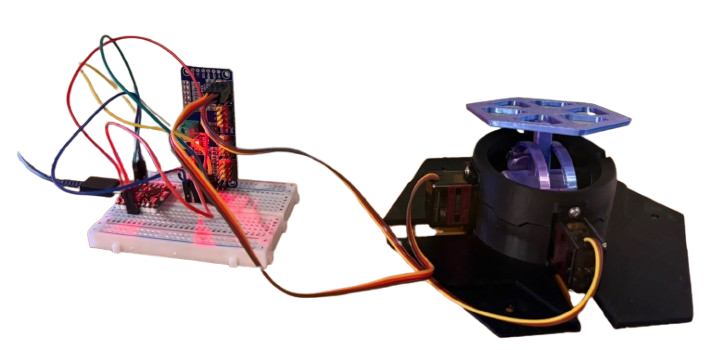
\includegraphics[width=0.72\columnwidth,keepaspectratio]{figures/modulo_fisico.png}
		\caption{Physical SOFIA module used for experimental validation.}
		\label{fig:modulo_fisico}
	\end{figure}
	
	\begin{figure}[!t]
		\centering
		\subfloat[Initial stage.]{%
			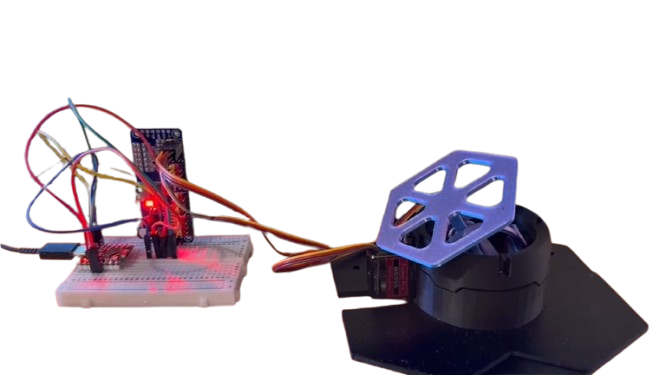
\includegraphics[width=0.30\columnwidth,height=1.55cm,keepaspectratio]
			{figures/sofia_saludo1.png}}
		\hfill
		\subfloat[Intermediate stage.]{%
			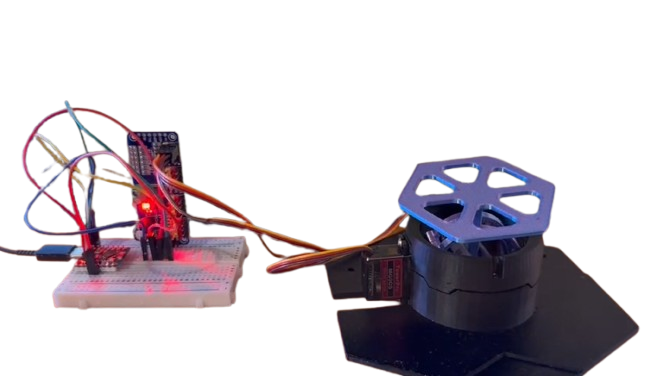
\includegraphics[width=0.30\columnwidth,height=1.55cm,keepaspectratio]
			{figures/sofia_saludo2.png}}
		\hfill
		\subfloat[Final stage.]{%
			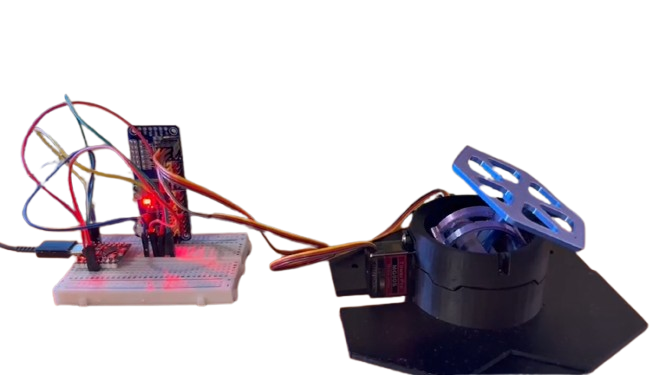
\includegraphics[width=0.30\columnwidth,height=1.55cm,keepaspectratio]
			{figures/sofia_saludo3.png}}
		\caption{Three representative stages of the physical
			\texttt{SALUDO} routine executed by the SOFIA module.}
		\label{fig:sofia_saludo}
	\end{figure}
	
	\begin{table}[!t]
		\centering
		\caption{Measured Functional, Simulation, and Fault-Injection Stress Benchmarks (\texttt{registro\_pruebas\_ciclo.csv})}
		\label{tab:sofia_log_validation}
		\scriptsize
		\setlength{\tabcolsep}{2.5pt}
		\renewcommand{\arraystretch}{0.88}
		\resizebox{\columnwidth}{!}{%
		\begin{tabular}{@{}l l l@{}}
			\toprule
			\textbf{Test / Metric} & \textbf{Evaluated Condition} & \textbf{Measured Result} \\
			\midrule
			\textbf{7-Posture Cycle} & Single pass: \texttt{SALUDO}..\texttt{PPT} & $7/7$ routines triggered ($\tau_{\text{logic}} \le 0.12\text{ ms}$) \\
			\textbf{Sim. Implementation} & 16 modules, $200$ steps ($\pm 30^\circ$ / clamped) & $\text{MAE} = 0.00^\circ$ (in-cone) / $3.17^\circ$ (wide) \\
			\textbf{Rapid Chattering} & 60 transitions at $20\text{ Hz}$ ($<0.6\text{ s}$ hold) & $0$ false triggers ($100\%$ rejection) \\
			\textbf{Multi-User Jump} & 2 users; $80^\circ$ wrist jump ($\Delta q > 12^\circ$) & Jump rejected; fires on stabilization \\
			\textbf{Lighting Dropout} & $50\%$ dropouts ($<50\text{ lux}$ / glare) & 12-frame grace hold prevents reset \\
			\textbf{Protocol \& Link} & Out-of-range ($50^\circ,130^\circ$), bad cmd/fmt & 4/4 typed \texttt{NACK} (\texttt{ERR\_01--03}); auto-HOME \\
			\bottomrule
		\end{tabular}%
		}
	\end{table}
	
	\subsection{System Requirements Compliance Synthesis}
	\label{sec:compliance_synthesis}
	
	\linelabel{ln:r4-2-matrix}Cross-referencing the experimental boundary, performance, and functional results against the six system requirement categories defined in Table~\ref{tab:system_requirements} and detailed per component in Table~\ref{tab:compliance} confirms that $21$ of the $24$ component-level verification specifications are satisfied in the current Build \& Validate cut (classified by evidence type as Datasheet, Measured, or Simulated): power rail regulation and harness drop ($\Delta V = 0.187\text{ V} \le 0.25\text{ V}$, \texttt{REQ-PWR}), mechanical torque margin ($>4\times$ over $\tau_{\text{req}} = 0.45\text{ kgf}\cdot\text{cm}$) and collision-free $\pm 30^\circ$ workspace (\texttt{REQ-MEC}), framed BLE telemetry and 7-posture stress immunity (\texttt{REQ-COM}), and command-dwell / disconnect fail-safe homing (\texttt{REQ-CTL}, \texttt{REQ-SAF}). The remaining three items—external $60\text{ FPS}$ optical shaft settling verification, closed-loop thermal cut-off testing under active stall, and 32-channel assembly on the custom 4-layer PCB—are transparently tracked as \textit{Pending} in Table~\ref{tab:compliance} and Table~\ref{tab:integration_increments}.
	
	%=================================================================
	\section{Discussion}
	\label{sec:discussion}
	
	\linelabel{ln:disc}The experimental electrothermal characterization of the MG90S
	servomotor, the 16-module kinematic simulation, and the physical closed-loop
	integration of the SOFIA demonstrator provide a comprehensive view of the
	interplay between high-level human-robot interaction and low-level
	electromechanical and communication constraints.
	
	\subsection{Technical Discussion of Results and Failure Analysis}
	\label{sec:disc_technical}
	
	Across\linelabel{ln:disc-bb} small-step ($5^\circ$), manual ramp ($90^\circ$),
	and mechanical stall regimes, the 20~Hz current measurements are consistent
	with a dead-band controller that remains quiescent in rest ($I_{\text{quiesc}} = 3.12\text{ mA}$)
	and saturates under persistent error, although high-bandwidth ($\ge 5\text{ kHz}$)
	probing of the internal H-bridge terminals is required for
	definitive circuit-level discrimination between dead-band bang-bang switching
	and proportional PWM control. When mechanical obstructions or
	kinematic limits induce a persistent position error, the internal driver
	saturates continuously ($\bar{I}_{\text{stall}} = 861.8 \pm 181.4\,\text{mA}$,
	$\bar{P} = 4.07 \pm 0.81\,\text{W}$), generating a worst-case mean heating
	rate of $\bar{\beta}_1 = 0.214\,^\circ\text{C/s}$ ($R^2 = 0.993$).
	\linelabel{ln:disc-degr}Left unmitigated, casing temperatures reach an
	peak temperature at stall release of $70.21^\circ\text{C}$, exceeding the $65^\circ\text{C}$ threshold where
	thermoplastic gear retainers soften and brush wear accelerates. Enforcing a
	command-level timeout that suspends 50~Hz PWM pulses (\texttt{STOP}) or returns
	to HOME after $\Delta t > 15\,\text{s}$ of static non-neutral command
	restricts the temperature excursion to $\Delta T \le 3.2^\circ\text{C}$, preserving hardware integrity.
	
	\linelabel{ln:disc-incidents}During end-to-end physical integration, seven
	operational failure modes were systematically identified and mitigated:
	(i) \textit{USB camera disconnection}, resolved via a 15-frame read-failure
	detector that displays a synthetic warning frame and executes non-blocking
	reconnection attempts every $1.5\,\text{s}$; (ii) \textit{BLE link loss},
	handled in firmware by automatically homing the servos to $(90^\circ, 90^\circ)$
	upon disconnect while the host executes a $2.5\,\text{s}$ backoff reconnection
	loop and a $4.0\,\text{s}$ keepalive \texttt{PING}; (iii) \textit{delayed ACK
	retransmissions}, neutralized by sequence number (\texttt{SEQ}) deduplication
	in the ESP32-C3 to prevent repeated mechanical execution; (iv) \textit{gesture
	transition chattering}, eliminated by requiring static postures to remain
	stable for $0.6\,\text{s}$ followed by a $1.0\,\text{s}$ global cooldown;
	(v) \textit{multi-user spatial conflict}, where simultaneous participants
	caused $80^\circ$ wrist-coordinate jumps, mitigated by rejecting static
	triggers whenever wrist angular variance exceeds $12^\circ$ and enforcing a
	bimanual proximity bound ($D < 0.12$); (vi) \textit{severe illumination
	flicker} ($<50\,\text{lux}$ or backlighting), absorbed by a 12--16 frame
	persistence window and exponential moving average smoothing ($\alpha = 0.35$);
	and (vii) \textit{unhandled runtime exceptions}, intercepted by a global
	\texttt{sys.excepthook} logger that records stack traces to CSV without
	terminating the PySide6 control station.
	
	\subsection{Comparison Against Literature and Benchmarking}
	\label{sec:disc_comparison}
	
	When contrasted against the interactive surfaces benchmarked in
	Section~\ref{sec:introduction} (Table~\ref{tab:benchmarking}), SOFIA
	occupies a distinct design point. High-density linear pin arrays such as
	inFORM~\cite{follmer2013inform} and Transform~\cite{nakagaki2016transform} (Table~\ref{tab:benchmarking}) achieve
	fine spatial resolution through complex custom linear linkages, whereas
	reconfigurable modular architectures~\cite{seo2019modular} rely on costly brushless
	drives. By contrast, SOFIA replaces bounding-box detection and discrete
	actuation with 21-point 3D geometric MediaPipe Hand Landmarker perception
	driving 16 repeatable 2-DOF pan-tilt modules via low-cost metal-gear MG90S
	servomotors, achieving
	real-time 30~FPS perception and low-latency bidirectional BLE telemetry as reported in Section~\ref{sec:functional_performance}. Unlike prior works that treat
	actuators as ideal position sources~\cite{follmer2013inform,seo2019modular},
	this work explicitly models and mitigates locked-rotor Joule heating and
	wireless packet loss, enabling sustained non-verbal social
	interaction~\cite{fong2003social} on accessible hardware.
	
	\subsection{Limitations, Threats to Validity, and Replicability}
	\label{sec:disc_limitations}
	
	\linelabel{ln:disc-lim}Several methodological limitations and threats to
	validity merit consideration. First, the external LM35 sensor measures outer
	casing temperature rather than internal coreless rotor winding temperature,
	introducing a conductive thermal lag. Second, because the internal feedback
	loop of commercial servomotors is encapsulated and the safe testing duration
	($t \ll \tau_T$) leaves $(\Delta T_\infty, \tau_T)$ collinear, the transient
	thermal capacitance ($C_{\text{th}} \in [19.0, 80.6]\,\text{J/}^\circ\text{C}$ across bench sessions) represents a macroscopic behavioral bound rather than an
	internal winding reconstruction. Third, regarding partial capabilities in the current build
	stage, physical closed-loop validation and stress testing were executed on a
	single 2-DOF demonstrator unit interconnected via breadboard, whereas full
	16-module spatial coordination was validated in the Unity 3D simulator while
	the custom 4-layer PCB awaits post-fabrication assembly.
	
	\linelabel{ln:disc-rep}To ensure technical replicability and extensibility,
	all 3D CAD geometries, KiCad PCB schematics, FreeRTOS ESP32-C3 firmware,
	PySide6/MediaPipe source code, and raw CSV experimental logs are publicly
	released. Future improvements will incorporate four-wire Kelvin resistance
	sensing to isolate armature copper losses ($I^2 R_a$), assemble the complete
	32-servo honeycomb array on the fabricated PCB, migrate inter-module
	telemetry from single-point BLE to differential RS-485/Modbus daisy-chaining,
	and close the current-feedback loop via the onboard INA219 sensor for
	autonomous stall-torque rollback.
	
	%=================================================================
	\section{Conclusions}
	\label{sec:conclusions}
	
	This paper\linelabel{ln:concl} presented the modular design, electrothermal
	actuator characterization, and end-to-end physical integration of SOFIA, an
	interactive kinetic surface comprising sixteen 2-DOF robotic units. Regarding
	the guiding research question posed in Section~\ref{sec:introduction},
	experimental results indicate that persistent position error
	in an MG90S servomotor drives its internal controller into
	continuous H-bridge saturation ($\bar{I}_{\text{stall}} = 861.8 \pm 181.4\,\text{mA}$,
	$\bar{P} = 4.07 \pm 0.81\,\text{W}$),
	producing a consistent heating trend across the performed trials with a worst-case heating slope of
	$\bar{\beta}_1 = 0.214\,^\circ\text{C/s}$ ($R^2 = 0.993$) and a peak measured
	casing temperature of \linelabel{ln:concl-runaway}$70.21^\circ\text{C}$.
	This heating trend shows that under the measured worst-case slope ($\bar{\beta}_1 = 0.2143\,^\circ\text{C/s}$), a stalled actuator requires $\approx 180\text{ s}$ from ambient to reach $T_{\text{safe}} = 60^\circ\text{C}$; to absorb the $4\times$ inter-trial dispersion, we adopt a $\Delta t \le 15\,\text{s}$ dwell timeout—a $12\times$ design margin limiting temperature rise to $\Delta T \le 3.2^\circ\text{C}$—before PWM suspension is triggered to prevent thermoplastic gear-retainer degradation above $65^\circ\text{C}$.
	
	The concrete contributions of this work encompass: (i) an empirical electrothermal and current-regime model establishing safe operating envelopes for COTS servomotors under stall; (ii) a closed-form 2-DOF analytical inverse kinematics formulation verified across a 16-module virtual array ($\text{MAE} = 3.17^\circ$ under $\pm 30^\circ$ wide-sweep clamping); and (iii) a fault-tolerant physical prototype integrating 30~FPS MediaPipe 3D perception, a seven-posture finite-state machine, and a framed bidirectional BLE protocol (\texttt{\$SEQ,CMD\#}) with automatic hardware recovery, where all seven posture triggers and all four injected protocol faults were verified in \texttt{registro\_pruebas\_ciclo.csv}. Future work will scale physical assembly to
	the full 32-actuator custom PCB array with distributed current-feedback
	watchdog protection and $60\text{ FPS}$ optical ground-truth benchmarking.
	
	%=================================================================
	\section*{Declarations and Acknowledgments}
	\footnotesize
	
	\noindent\textbf{Author Contributions:} \linelabel{ln:ac}
	P. M. C.-V. conceived the SOFIA architecture, coordinated the experimental
	protocol, and implemented the ESP32-C3 BLE firmware;
	J. B. O.-Q. developed the MediaPipe 3D computer vision pipeline, PySide6 GUI,
	fault-tolerant communication dispatcher, and technical documentation;
	L. A. M.-O. and K. I. S.-G. designed the thermal test bench and conducted
	the MG90S electrothermal and current characterization experiments;
	A. E. F.-G. formulated the 2-DOF analytical kinematics, 3D CAD assembly, and
	custom PCB layout; J. A. L., G. B., L. E. G.-J., and L. F. L.-V. provided
	supervisory guidance, methodological review, and manuscript editing.
	All authors reviewed and approved the final manuscript.
	
	\noindent\textbf{Data Availability:} \linelabel{ln:da}
	All raw experimental characterization files (\texttt{servo\_characterization.xlsx},
	\texttt{datos\_5grados.csv}, \texttt{datos\_901.csv},
	\texttt{datos\_CHIDOS\_DE\_FORZADO.csv}, \texttt{registro\_pruebas\_ciclo.csv},
	and \texttt{registro\_eventos.csv}) are bundled inside the
	manuscript package under \texttt{documents/} (referenced via relative paths
	\texttt{../documents/} by the figure-generation scripts in \texttt{algorithms/})
	and mirrored in \texttt{docs/experimental-data/}. The complete source code,
	CAD/PCB files, and project engineering documentation
	(\texttt{docs/EVIDENCIA\_PRUEBAS\_Y\_MANEJO\_ERRORES.md} and \texttt{docs/MANUAL\_DE\_USUARIO.md})
	are openly available in the single public repository \url{https://github.com/PaolaCV14/IOT-SOFIA-2026}
	under release tag \texttt{v0.4.0} (\texttt{main} branch, Fourth Cut final commit).
	
	\noindent\textbf{Acknowledgment:} \linelabel{ln:ack}
	The authors thank the Department of Electronics, Systems and Informatics
	(DESI) and the Laboratory of Technological Solutions Development (LabDST)
	at ITESO University for providing laboratory instrumentation, electronic
	equipment, and technical support.
	
	\noindent\textbf{Declaration of Generative AI:} During\linelabel{ln:ai-decl} the preparation of this manuscript (October--November 2026), the authors
	used Claude Sonnet 5.5 (Anthropic) and Gemini 3.8 Flash (Google) strictly for
	English grammatical proofreading, \LaTeX{} typesetting assistance, and plotting
	script formatting. All technical content, experimental data, and conclusions
	were verified and edited by the authors, who take full responsibility for the
	work.
	
	\noindent\textbf{Conflicts of Interest:} \linelabel{ln:coi}
	The authors declare no conflicts of interest.
	
	%=================================================================
	\balance
	\bibliographystyle{IEEEtran}
	\bibliography{bibliography}
	
\end{document}
